%\documentclass[german,a4paper,12p,headsepline, titlepage, liststotoc, idextotoc,bibtoctoc,blibliography = totocnumbered,left=40mm,right=20mm,top=25mm,bottom=20mm]{scrartcl}
\documentclass[german,a4paper, 12pt]{llncs}
\usepackage[left=30mm,right=30mm,top=25mm,bottom=25mm]{geometry}
\setlength{\footskip}{6mm} % Abstand Seitenzahl zu Text
\setcounter{tocdepth}{2}
\makeatletter
\renewcommand*\l@author[2]{}
\renewcommand*\l@author[2]{}
\makeatletter
\usepackage[utf8]{inputenc}
\usepackage[backend=biber,sorting =none]{biblatex}
\usepackage{csquotes}
\usepackage{graphicx}
\usepackage{babel}
\usepackage{subcaption}
\usepackage{mwe}
\usepackage[toc, page]{appendix}

\usepackage{parskip}
\usepackage{float}
%\usepackage{hbrs-inf}

%\usepackage{hyperref}
\usepackage{filecontents}


\begin{filecontents}{references.bib}
	

@article{averageHairshedding,
	author = {Sinclair, Rodney},
	year = {2015},
	month = {04},
	pages = {},
	title = {Hair Shedding In Women: How much is too much?},
	volume = {173},
	journal = {The British journal of dermatology},
	doi = {10.1111/bjd.13873}
}

@article{visualScale,
	author = {Martínez-Velasco, María and Vázquez-Herrera, Norma and Maddy, Austin and Asz-Sigall, Daniel and Tosti, Antonella},
	year = {2017},
	month = {02},
	pages = {},
	title = {The Hair Shedding Visual Scale: A Quick Tool to Assess Hair Loss in Women},
	volume = {7},
	journal = {Dermatology and Therapy},
	doi = {10.1007/s13555-017-0171-8}
}

@article{seasoalShedding,
	
	author = {Hsiang, E.Y. and Semenov, Yevgeniy and Aguh, Crystal and Kwatra, S.G.},
	year = {2017},
	month = {10},
	pages = {},
	title = {Seasonality of hair loss: a time series analysis of Google Trends data 2004 to 2016},
	volume = {178},
	journal = {British Journal of Dermatology},
	doi = {10.1111/bjd.16075}
}

@inbook{chemicalAlopecia,
	author = {Maibach, Howard and Yamaguchi, Ian},
	year = {2012},
	month = {01},
	pages = {1935-1942},
	title = {Chemically Induced Hair Loss/Alopecia},
	isbn = {978-3-642-02034-6},
	journal = {Kanerva's Occupational Dermatology, Second Edition},
	doi = {10.1007/978-3-642-02035-3_205}
}

@article{ironDeficiency,
	author = {Trost, Leonid and Bergfeld, Wilma and Calogeras, Ellen},
	year = {2006},
	month = {06},
	pages = {824-44},
	title = {The diagnosis and treatment of iron deficiency and its potential relationship to hair loss},
	volume = {54},
	journal = {Journal of the American Academy of Dermatology},
	doi = {10.1016/j.jaad.2005.11.1104}
}

@ONLINE{Canny,
	title = {Canny Edge Detector},
	url = {https://docs.opencv.org/master/da/d5c/tutorial_canny_detector.html},
	urldate = {2020-04-17},
}

@article{Watershed,
	author = {Kornilov, Anton and Safonov, Ilia},
	year = {2018},
	month = {10},
	pages = {123},
	title = {An Overview of Watershed Algorithm Implementations in Open Source Libraries},
	volume = {4},
	journal = {Journal of Imaging},
	doi = {10.3390/jimaging4100123}
}

@ONLINE{WatershedCV,
	title = {Image Segmentation with Watershed Algorithm},
	url = {https://opencv-python-tutroals.readthedocs.io/en/latest/py_tutorials/py_imgproc/py_watershed/py_watershed.html},
	urldate = {2020-04-17}
}

@ONLINE{TemplateMatchingCV,
	title = {Template Matching},
	url = {https://docs.opencv.org/2.4/doc/tutorials/imgproc/histograms/template_matching/template_matching.html},
	urldate = {2020-04-17}
}

@ONLINE{Matplotlib,
	title = {Matplotlib},
	url = {https://matplotlib.org/},
	urldate = {2020-04-17}
}

@ONLINE{Numpy,
	title = {Numpy},
	url = {https://numpy.org/},
	urldate = {2020-04-17}
}

@ONLINE{DilationCV,
	title = {Eroding and Dilating},
	url = {https://docs.opencv.org/2.4/doc/tutorials/imgproc/erosion_dilatation/erosion_dilatation.html},
	urldate = {2020-04-17}
}

@ONLINE{ConnectedComponents,
	title = {Connected Components in OpenCV},
	url = {https://davidlavy.wordpress.com/opencv/connected-components-in-opencv/},
	urldate = {2020-04-17}
}

@ONLINE{skel,
	title = {Skeletonize},
	url = {https://scikit-image.org/docs/dev/auto_examples/edges/plot_skeleton.html},
	urldate = {2020-04-17}
}

@inproceedings{outlierRemoval,
	author = {Amidan, B.G. and Ferryman, Thomas and Cooley, Scott},
	year = {2005},
	month = {04},
	pages = {3814 - 3819},
	title = {Data outlier detection using the Chebyshev theorem},
	journal = {Proc. IEEE Aerosp. Conf.},
	doi = {10.1109/AERO.2005.1559688}
}

@ONLINE{curveFittingIntro,
	title = {Introduciton to Curve Fitting},
	url = {https://www.ncss.com/wp-content/themes/ncss/pdf/Procedures/NCSS/Introduction_to_Curve_Fitting.pdf},
	urldate = {2020-04-17}
}
@ONLINE{curveFittingScipy,
	title = {scipy curve fit},
	url = {https://docs.scipy.org/doc/scipy/reference/generated/scipy.optimize.curve_fit.html},
	urldate = {2020-04-17}
}
@ONLINE{splineScipy,
	title = {scipy InterpolatedUnivariateSpline},
	url = {https://docs.scipy.org/doc/scipy/reference/generated/scipy.interpolate.InterpolatedUnivariateSpline.html},
	urldate = {2020-04-17}
}


\end{filecontents}

\addbibresource{references.bib}
\title{Praxisprojekt}
\subtitle{Automatisches Schätzen der Haaranzahl in ausgefallenen Haarbüscheln}
\author{\parbox{.9\textwidth}{\centering 
		\large Janelle Pfeifer \\
		\small Delpstraße 28\\
		53359 Rheinbach \\
		janelle.pfeifer@smail.inf.h-brs.de}}
\institute{\parbox{.9\textwidth}{\centering 
		\large Hochschule Bonn-Rhein-Sieg \\
		\normalsize Institute of Visual Computing \\ 
		\small Fachbereich Informatik \\
		Studiengang: Informatik (B.SC.)\\
		\normalsize Rheinbach, 24.4.2020}}
\date{Rheinbach, 24.4.2020}

\begin{document}
	%{\let\newpage\relax\maketitle}
	\maketitle
	\newpage
	\tableofcontents
	\newpage

\begin{abstract}
	am ende hier ein abstract hin
\end{abstract}

\section{Einleitung}
%Die Einleitung ist mit der wichtigste Teil der Arbeit, da sie den Leser motivieren soll die vorliegende Arbeit weiter z lesen. Sie sollte neben einer Motivation bzw Problembeschreibung auch das Ziel der Arbeit beschreiben.Zusätzlich sollten die Fabgebiete die die arbeit betreffen und deren Bedeutung genannt werden. Wichtig ist eine klare Formulierung der Zielstellung und des Lösungsansatzes so wie abschließend eine Beschreibung der Gliederung der Arbeit.

Das Ausfallen von Haarsträhnen ist ein natürlicher Teil des Haarwachstum-Zyklus. Durchschnittlich verliert der Mensch 50 bis 150 Haarsträhnen am Tag. Vermehrter Haarverlust kann ein Anzeichen von Krankheiten oder Mangelerscheinungen sein.\cite{averageHairshedding}

Haarausfall ist sehr variabel und wird durch viele Faktoren beeinflusst. Er kann sich abhängig von dem Haartyp, der Haarlänge und der Haarpflege-Methode jeden Tag ändern und Muster aufweisen. Jeder Mensch hat ein eigenes Haarausfall-Muster. Eine Langzeitüberwachung gibt die Möglichkeit diese Muster zu erkennen und Abweichungen herauszustellen. \cite{chemicalAlopecia,ironDeficiency,seasoalShedding}

In dem Paper \blockquote{The Hair shedding visual scale: A quick tool to assess hair loss in Women} wird eine Methode beschrieben, in der Frauen anhand von Bildern den Umfang ihres täglichen Haarausfalls bestimmen können. Dabei werden den Frauen Bilder von abgezählten, ausgefallenen Haarbüscheln gezeigt, die ihrer eigenen Haarlänge entsprechen. Die Frauen wählen das Foto aus, welches ihrem persönlichen täglichen Haarausfall entspricht. Dabei wurde eine Korrelation festgestellt zwischen Frauen, die klinisch bestätigt Haarverlust erfahren und den Bildern, die sie auswählen.
Der Haarausfall kann somit visuell, anhand von Bildern festgestellt werden.\cite{visualScale}

In dieser Arbeit wird ein Verfahren vorgestellt, mit dem der tägliche Haarausfall mithilfe von Methoden der Bildverarbeitung und statistischer Auswertung geschätzt werden kann. So wird eine Langzeitüberwachung möglichst effizient durchführbar.
\section{Grundlagen}
\subsection{Computervision}
In dem Bereich der Bildverarbeitung gibt es viele Algorithmen, die es ermöglichen Objekte in einem Bild erkennbar zu machen und zu verarbeiten.

\subsection{Template Matching} 

Template Matching findet Bereiche eines Bildes, die einem gegebenen Bildteil, einem Template, ähnlich sind.

Dazu wird ein Source Image und ein Template Image angegeben. Um die gesuchten Bereiche zu finden, wird das Template Image Pixelweise über das Source Image geschoben. An jeder Stelle wird das Template mit dem Source Image verglichen und die Ähnlichkeit zwischen den Beiden berechnet. Als Ergebnis erhält man eine Matrix die für jeden Pixel des Bildes eine Wahrscheinlichkeit dafür angibt, das sich dort das Template befindet.\cite{TemplateMatchingCV}

\subsection{Canny Edge Detection}
Canny Edge Detection ist ein Algorithmus der Kanten in einem Bild erkennt. 
Es handelt sich um einen Hochpassfilter. Diese suchen nach Stellen im Bild, wo sich die Farben bzw. Graustufen stark voneinander unterscheiden. Solche Stellen heißen Hochfrequent. Linien und Kanten weise eine Hohe Frequenz auf. Niederfrequente Bereiche weisen eine einheitlichere Farbe oder Graustufe auf.\cite{Canny}

Ein Hochpassfilter lässt hochfrequente Bildanteile stehen und schwächt Niederfrequente ab. 
Canny Edge Detection wird auf Graustufenbilder angewandt. An jeder Stelle des Bildes wird ein 3x3 Ausschnitt der Nachbarpixel betrachtet. Weisen die Nachbarpixel ein Bestimmtest Muster auf, indem der Graustufe-unterschied eine Linie beschreibt mit Helleren Pixel auf einer Seite und dunkleren Pixeln auf der anderen, wird die Stelle als Teil einer Kante betrachtet.\cite{Canny}


\subsection{Dilatation}
Die Dilatation arbeitet auf binären Bildern. Es gibt nur schwarz und weiß.
Die Dilatation fügt weiße Pixel an die Ränder von weißen Objekten hinzu. 
Bei der Dilatation handelt es sich um ein Morpholigschen Operator. Diese arbieten das Bild Pixelweise durch. Der Wert jedes Pixels basiert auf einem Vergleich zischen dem Pixel und dessen Nachbar-Pixeln.\cite{DilationCV}
	
\subsection{Inversion eines Graustufenbildes}

Die Graustufenwerte eines Bildes werden invertiert. 
Schwarz wird Weiß und Weiß wird Schwarz, helle Graustufen werden dunkel und umgekehrt.
 
Die Graustufen eines Bildes werden in 8 bit dargestellt. Somit gibt es 255 Graustufen. 0 ist schwarz und 255 ist weiß. 
Somit gilt bei der Inversion für jedes Pixel mit dem Graustufenwert g:
g_{neu} = 255- g_{alt} 

\subsection{Watershed Algorithmus}

Der Watershed Algorithmus ist ein Region Growth Algorithmus. Er finden zusammenhängende Gruppen an Pixeln, die einander ähnlich sind. Diese Gruppen werden als Regionen bezeichnen. 

Für den Watershed Algorithmus wird zunächst in jede Region, die der Algorithmus wachsen lassen soll, eine Markierung, ein seed, gesetzt.
Für die seeds werden die Pixel, die dem seed ähnlich sind zu der Region zusammengefasst. So wachsen die Regionen, bis sie auf eine andere Region stößt.

Das Prinzip ist es die Graustufenwerte des Bildes als eine Topologische Karte anzusehen. Jeder seed liegt in einem Tal, in das Wasser hineingefühlt wird. 
Die Grenzen zwischen den Regionen liegen dort, wo das Wasser aus unterschiedlichen Tälern aufeinander trifft.\cite{Watershed,WatershedCV} 

\subsubsection{Region Growth}
ist ein Verfahren, bei dem ein Bild in Regionen unterteilt wird. So werden zum Beispiel Sektionen mit ähnlicher Farbe herausgestellt.

\subsection{Connected Components}

Connected Components sind benachbarte Pixel, die denselben Grauwert haben. \cite{ConnectedComponents}

\subsection{Skelettierung}
Bei der Skelettierung werden Objekte in einem Bild auf nur eine Pixelbreite reduziert. Dabei Gelten Objekte als Connected Components. So können Linien auf eine Pixelbreite geschrumpft werden.\cite{skel}

\subsection{Outlier Removal}

Ein Algorithmus der statistische Ausreißer entfernt. 
Basierend auf dem Tschebyscheff Theorem, wird der Mittelwert und die Varianz eines Satzes von Messdaten verwendet, um Ausreißer zu erkennen.\cite{outlierRemoval}

\subsection{Fitted Curve, lineare Regression, Spline}

Eine Fitted Curve ist eine mathematische Funktion, die Messdaten in einem Zeit Dimensionalem Raum am besten abbildet.


Um Messdaten mit einer Funktion Approximieren zu können, wird eine Funktionstyp vorgegeben, die dann an die Daten angepasst wird. 
Beispielsweise eine Ganzrationale Funktion, eine exponentielle Funktion oder eine logarithmische Funktion. 

Die Lineare Regression ist eine Fitted Curve mit einer linearen Funktion.\cite{curveFittingIntro,curveFittingScipy}

Eine Spline ist eine Kurve, die durch ausgewählte, oder alle Messdaten verläuft. Sie kann mithilfe von Interpolation berechnet werden.\cite{splineScipy}

\section{Design und Implementation}

Das Ziel ist es die Einschätzung eines Haarbüschels, mithilfe von Computervision, zu automatisieren. Zunächst wird ein Kalibriervorgang durchgeführt, in dem der Nutzer abgezählte Haarbüschel-Bilder eingibt. Dann kann die Menge der Haare in nicht abgezählten Haarbüscheln automatisch geschätzt werden.

Die Schätzungen werden zugehörig zum Datum gespeichert. Um einen Zeitlichen verlauf festzuhalten.
Zusätzlich zu den Schätzungen kann für jedes Datum eine Marker angegeben werden. So können regelmäßige Wiederholungen der Haarpflege, wie zum Beispiel eine Haarwäsche, notiert werden. Des weiteren können gesundheitliche Veränderungen oder Einnahme von Medikamenten vermerkt werden.

Das Programm wurde in Python implementiert und nutzt unter anderem das Plugin Open-cv.
Der Nutzer steuert das Programm über die Kommandozeile. 

Da die Haare jeder Person unterschiedlich sind, muss für jeden Nutzer eine eigene Kalibrierung durchgeführt werden. Um Vermischung von Daten unterschiedlicher Personen und häufige Neukalibrierungen zu vermeiden, kann das Programm beliebig viele Nutzer anlegen und verwalten. 

\subsection{Verarbeitung der Haar-Bilder}

Sowohl für die Kalibrierung als auch für die Schätzung von Haar-Mengen müssen die eingegebenen Bilder zunächst verarbeitet werden und Daten, mit denen auf die Haar-Menge geschlossen werden kann herausgestellt werden. Dazu werden Methoden der Bildverarbeitung verwendet.

Die Methode detect implementiert die Verarbeitung eines Bildes.
Als Eingabe wird von einem Haarbüschel auf einem einfarbige Hintergrund ausgegangen. Dabei sollte ein möglichst guter Kontrast zu der Haarfarbe gewählt worden sein. Beispielsweise ein weißer Hintergrund für dunkele haare oder ein schwarzer Hintergrund für blondes oder hellbraunes Haar. Die Ecken des Hintergrundes sind durch ein Symbol markiert. Vergleich Abbildung \ref{img:input}.

\begin{figure}[H]
	\centering
	
\includegraphics[width=0.6\textwidth]{fig64/00IMG_20200406_153354_12_g_15.jpg}
	\caption[]{Input}
	\label{img:input}
\end{figure}

Im ersten Schritt der Bildverarbeitung wird das Bild auf die Markierungen in den Ecken zugeschnitten. Das ist in der Methode cropDots implementiert.
Über einen Aufruf der Open cv methode matchTemplate wird nach vorkommen der Markierung gesucht. Das Resultat ist ein Karte an Wahrscheinlichkeiten, die für jedes Pixel angibt, zu welcher Wahrscheinlichkeit sich dort die Markierung befindet. Die 4 Stellen an denen die Wahrscheinlichkeit am höchsten ist, werden als Eckpunkte angesehen. Siehe Abbildung \ref{img:cropDots}.\cite{TemplateMatchingCV}
\begin{figure*}
	\centering
	\begin{subfigure}[b]{0.475\textwidth}   
		\centering
		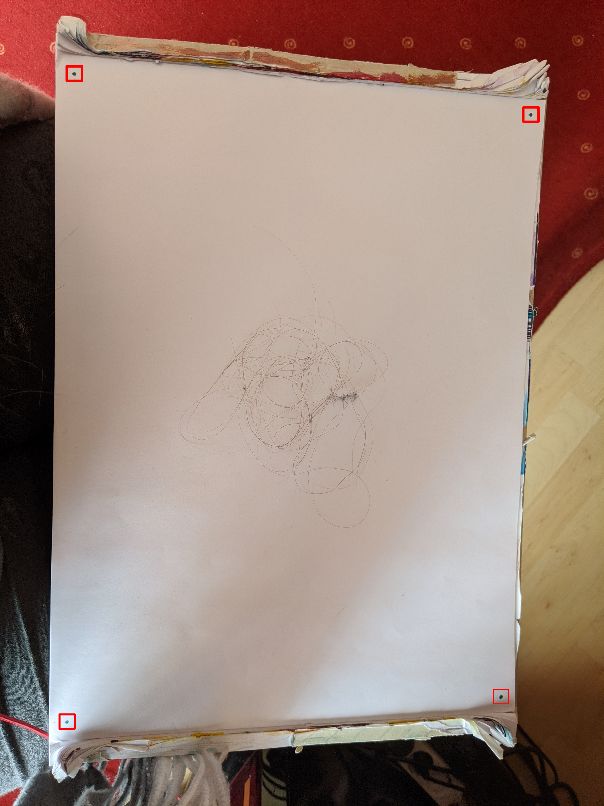
\includegraphics[width=\textwidth]{fig64/03rectImg.png}
		\caption[]{Die 4 erkannten Markierungen im Bild}
		\label{img:foundDots}
	\end{subfigure}
	\quad
	\begin{subfigure}[b]{0.475\textwidth}   
		\centering
		
\includegraphics[width=0.9\textwidth]{fig64/03crop image.png}
		\caption[]{Resultat des Zuschneidens}
		\label{img:Crop}
	\end{subfigure}
	\caption[ der Prozess des Zuschneidens auf Markierungen in den Ecken ]
	{\small Der Prozess des Zuschneidens auf Markierungen in den Ecken} 
	\label{img:cropDots}
\end{figure*}


Durch das Zuschneiden der Bilder wird sichergestellt, das die Haare immer etwa einen gleichgroßen Hintergrund haben. So werden die Daten, die aus den Bildern gezogen werden, nicht verfälscht dadurch, das die Haare eventuell von unterschiedlichen Abständen fotografiert wurden. 

Nach dem Zuschneiden werden die Haare von dem Hintergrund getrennt.
Das ist in der Methode edgeProcess implementiert. 
Mithilfe von Canny Edge detection werden die Haare grob erkannt.
Weiße Pixel gelten als Haare, schwarze als Hintergrund. Siehe Abbildung \ref{img:Edges}.
\begin{figure*}
	\centering
	\begin{subfigure}[b]{0.475\textwidth}
		\centering
		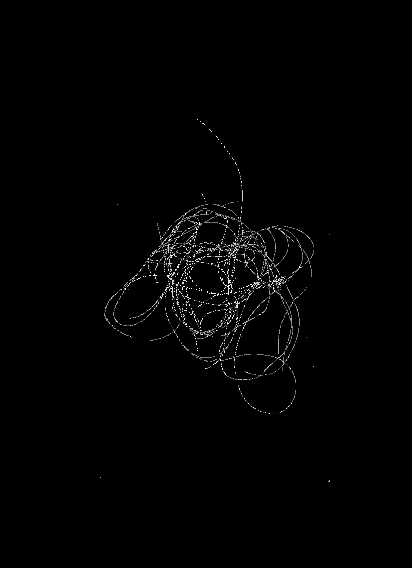
\includegraphics[width=\textwidth]{fig64/04edges.png}
		\caption[]{Canny Kantendetektion}
		\label{img:Edges} 
	\end{subfigure}
	\hfill
	\begin{subfigure}[b]{0.475\textwidth} 
		\centering
		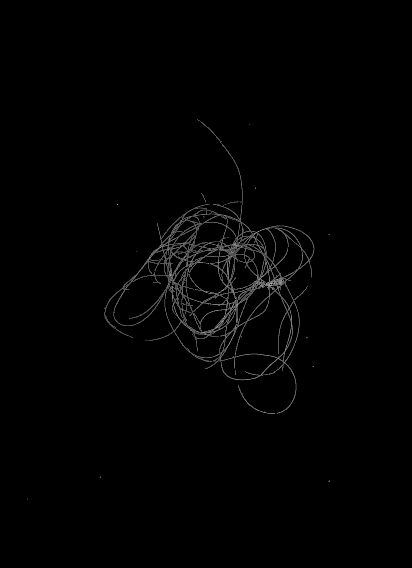
\includegraphics[width=\textwidth]{fig64/05intenstiy.png}
		\caption[]{Intensität-Abbildung der Haare}
		\label{img:Intensity}
	\end{subfigure}
	\caption[  ]
	{\small Beispiel input von knielangen dunkelroten Haare} 
	\label{img:cannywrap}
\end{figure*}


In der Methode hairPixelIntensity wird die Detektion verfeinert.
Auf das Resultat der Kantendetektion wird eine Dilatation ausgeführt. Dadurch gelten mehr Pixel als Haare und eventuelle Löcher wachsen zusammen.

Da Haare halb-transparent sind, wird ihre Farbe intensiver, wenn sie sich überlagern. Sie weisen eine höhere Intensität auf.
Um die Haar-Intensität des Bildes zu extrahieren, wird ein Bild gebaut, in dem Hintergrund Pixel weiß sind, und Haarpixel ihren Graustufenwert aus dem Original Bild erhalten.

Wenn die Haare heller sind als der Hintergrund, es sich beispielsweise um blondes Haar auf schwarzem Hintergrund handelt haben die Haare eine Höhere Intensität, wenn sich heller sind. Bei dunklem Haar auf hellem Hintergrund ist es gegenteilig. Die Intensität ist höher, wenn das Haar dunkler ist.
Damit beide Konstellationen zu einem ähnlichen Ergebnis kommen, werden die Graustufen invertiert, wenn die Haare hell sind. So ist auch bei ursprünglich hellem Haar, die Intensität höher, wenn die Graustufen dunkler sind.



Die Inversion dieses Bildes ergibt ein Bild mit schwarzem Hintergrund und Haaren, die Heller sind an stellen wo sie sich Überlagern. Siehe Abbildung \ref{img:Intensity}.


Es werden kleine vereinzelte Gebiete des Hintergrundes in der Kantendetektion erkannt und gelten somit als Haare.
Um diese Gebiete zu erkennen und zu entfernen, wird der Watershed Algorithmus angewendet.   
Dabei werden Marker in alle verbundenen Gebiete gesetzt, die nicht schwarz sind. Der Watershed Algorithmus lässt die Regionen wachsen. 
Dann werden die Regionen entfernt, die im Verglich auf die Größe des Bildes sehr klein sind. Siehe Abbildung \ref{img:smallRegionwrap}.

Die Summe aller Graustufenwerte werden als Intensität gespeichert. Dabei wird der Hintergrund außer Acht gelassen, weil es schwarz ist, und somit den Graustufenwert 0 hat.
\begin{figure*}
	\centering
	\begin{subfigure}[b]{0.475\textwidth}
		\centering
		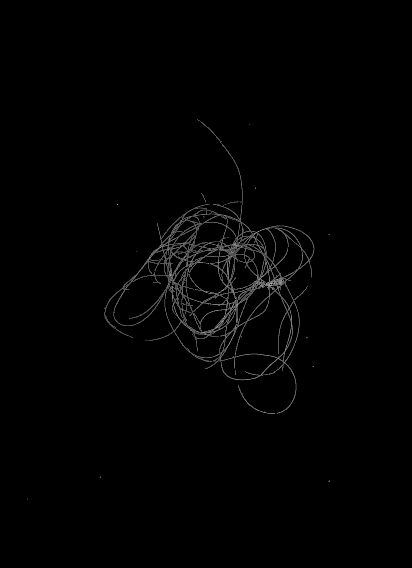
\includegraphics[width=\textwidth]{fig64/05intenstiy.png}
		\caption[]{Intensität-Abbildung der Haare}
		\label{img:Intensity2}
	\end{subfigure}
	\hfill
	\begin{subfigure}[b]{0.475\textwidth} 
		\centering
		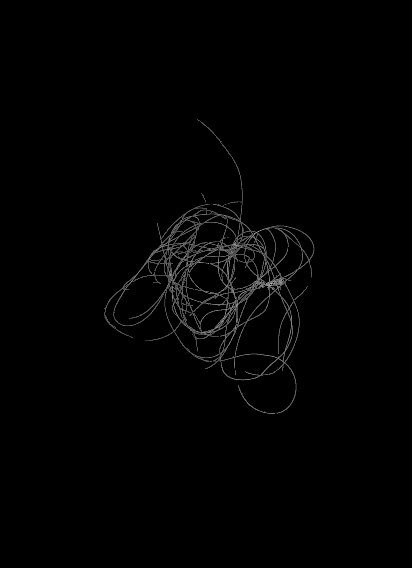
\includegraphics[width=\textwidth]{fig64/06small regions removed.png}
		\caption[]{Kleine Regionen Entfernt}
		\label{img:smallRegion}
	\end{subfigure}
	\caption[  ]
	{\small Enternen von kleinen Regionen, vorher nachher} 
	\label{img:smallRegionwrap}
\end{figure*}

In der Methode hairPixelPercentage werden die Pixel gezählt die als Haare gelten. Zusätzlich wird der Prozentsatz an Haar Pixeln und die Intensität des Bildes im Vergleich zur Bildgröße gespeichert. 

Dann wird die Dichte der Haare Untersucht. In der Methode 
Dafür werden die Hintergrund Regionen bestimmt, die durch Haare getrennt werden. Dafür wird der Watershed Algorithmus angewendet.
Die Marker werden in alle zusammenhängenden Hintergrundgebiete gesetzt.
Dabei wird die Größe der Region, die die Haare umschließt gespeichert. Abbildung \ref{img:outerSection}.
Zusätzlich wird die Anzahl der Regionen die von Haaren umschlossen wird und deren Durchschnittliche Größe gespeichert.\cite{Watershed,WatershedCV}
\begin{figure*}
	\centering
	\begin{subfigure}[b]{0.475\textwidth}
		\centering
		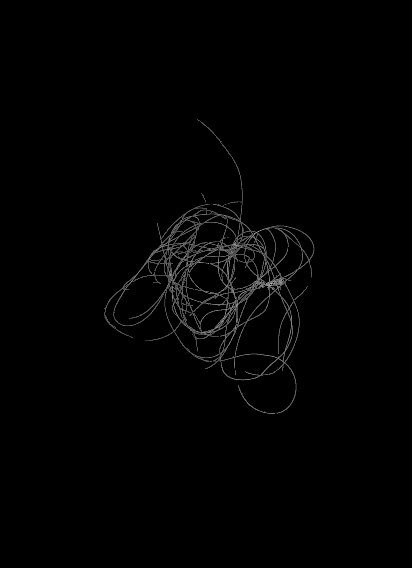
\includegraphics[width=\textwidth]{fig64/06small regions removed.png}
		\caption[]{watershed input}
		\label{img:wsiput}
	\end{subfigure}
	\hfill
	\begin{subfigure}[b]{0.475\textwidth} 
		\centering
		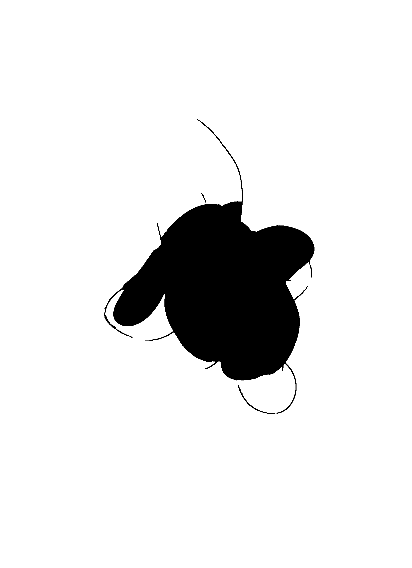
\includegraphics[width=\textwidth]{fig64/08outer section.png}
		\caption[]{Äußerte Region Isoliert und in weiß dargestellt.}
		\label{img:outerSection}
	\end{subfigure}
	\caption[  ]
	{\small Anwendung von Watershed} 
	\label{img:regionwrap}
\end{figure*}

Als nächstes werden die Gebiete des Bildes untersucht, die eine erhöhte Haar-Dichte aufweisen.
Dafür wird das Intensität-Bild skelettiert. Siehe Abbildung \ref{img:skel}.
Die Hintergrund Regionen werden wie zuvor untersucht.

\begin{figure*}
	\centering
	\begin{subfigure}[b]{0.475\textwidth}
		\centering
		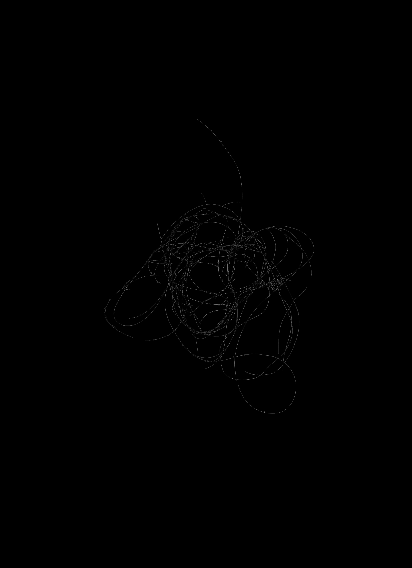
\includegraphics[width=\textwidth]{fig64/09input intensity.png}
		\caption[]{Skelett des Intensität-Bildes}
		\label{img:skel}
	\end{subfigure}
	\hfill
	\begin{subfigure}[b]{0.475\textwidth} 
		\centering
		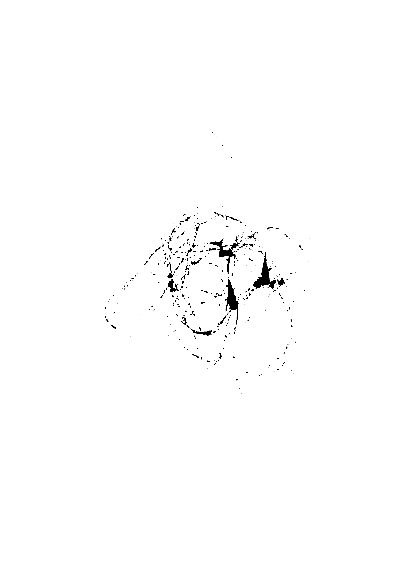
\includegraphics[width=\textwidth]{fig64/09outer section.png}
		\caption[]{Äußerte Region des skelettierten Bildes}
		\label{img:skelBGregion}
	\end{subfigure}
	\caption[  ]
	{\small Dichtere Regionen untersuchen} 
	\label{img:skelwarp}
\end{figure*}

In der Methode denseAndLoosePerc wird die Haar-Intensität in den dichteren Regionen und in den weniger dichten Regionen berechnet und abgespeichert.

Für das Bild werden 28 Datenpunkte extrahiert und abgespeichert. Siehe Anhang \ref{appendix:datenpunkte}. 



\subsection{Kalibrieren}

Die Kalibrierung ist in der Methode calibration implementiert.
Für die Kalibrierung werden mehrere Bilder als Input angegeben. Für jedes der Bilder wird die Menge der Haare in dem Titel des Bildes angegeben. 
Die Bilder werden alle mit detect Untersucht. Die Daten aus den Untersuchungen, sowie die Haar-Mengen werden abgespeichert.
ganzen Ordner kalibrieren. einzelne Bilder hinzufügen.

\subsection{Relation Daten zu Haar Menge}



\subsection{Schätzen eines Haar-Bildes}

Nachdem eine Kalibrierung durchgeführt wurde. Kann die Haar-Menge auf beliebigen Bildern geschätzt werden.
Das Schätzen ist in der Methode readFilesAndGuess implementiert.

Zuerst wird das zu schätzende Bild mithilfe von detect Untersucht.
Dann werden die Daten aus der Kalibrierung geladen. 
Die Daten werden teilweise miteinander verrechnet und dann auf die dazugehörigen Haar-Mengen abgebildet.
So entstehen eine Menge an Graphen, bei denen die Haar-Menge jeweils auf der y Achse liegt. Siehe Abbildung \ref{fig:mapping}. 

\begin{figure}
	\centering
	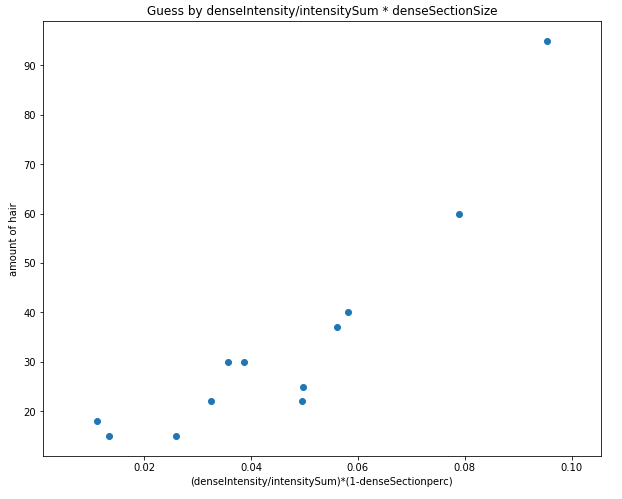
\includegraphics[width=0.8\textwidth]{fig64/gh4.PNG}
	\caption[]{Haar-Menge in Relation zur Intensität in dichten Regionen normalisiert durch gesamte Intensität und Region-Größe}
	\label{fig:mapping}
\end{figure}

Die Punkte in den Graphen werden durch Funktionen Approximiert. Die Funktionen können dann genutzt werden um Haar-Mengen zu schätzen.
Für jeden Graph werden 3 Funktionen berechnet. Eine Lineare Regression, eine Spline-Interpolation, und eine benutzerdefinierte Funktion.
Der Benutzer kann aus linear, logarithmisch und exponentiell aussuchen.
Siehe Abbildung \ref{fig:func}.

\begin{figure}
	\centering
	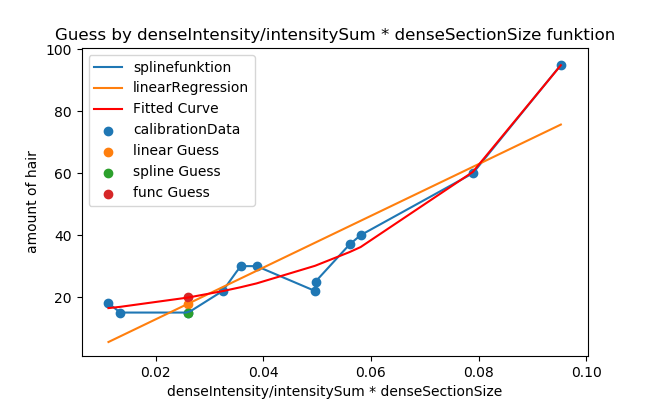
\includegraphics[width=0.9\textwidth]{fig64/g11_denseIntensitynormDetailed.png}
	\caption[]{Funktionen, die Datenpunkte Approximieren. Spline-Interpolation, lineare Regression und exponentielle Funktion.}
	\label{fig:func}
\end{figure} 

Von den 28 Datenpunkten die aus den Bildern ausgewertet werden, werden 17 Genutzt um 12 Modelle zu erstellt. Diese Modelle wurden als aussagekräftig gefunden, um die Haarmenge schätzen zu können. Untersucht werden die Menge der Pixel, die als Haare zählen, Intensität, Größe und Anzahl an Hintergrund-Regionen. Siehe Anhang \ref{appendix:xwertemodel} Für die Berechnungen der genutzten x Werte für die Modelle. 

Siehe den Anhang \ref{appendix:modelle} für die graphische Darstellung der Modelle.

Für jedes der Modelle werden 3 Funktionen approximiert. Mit den Funktionen werden jeweils 3 Schätzungen für das zu schätzdene Bild berechnet. 

Ausreißer werden entfernt. Dazu werden zunächst alle Schätzungen von weniger als 0 Haaren entfernt. Zusätzlich werden statistische Ausreißer mithilfe eines Algorithmus basierend auf dem Tschebyscheff Theorem entfernt.\cite{outlierRemoval}

Der Mittelwert, der übrig gebliebenen Schätzungen, ist das Endergebnis. 
Siehe Abbildung \ref{img:guess} für den Verlauf einer Schätzung auf der Kommandozeile.

\begin{figure}
  \centering
  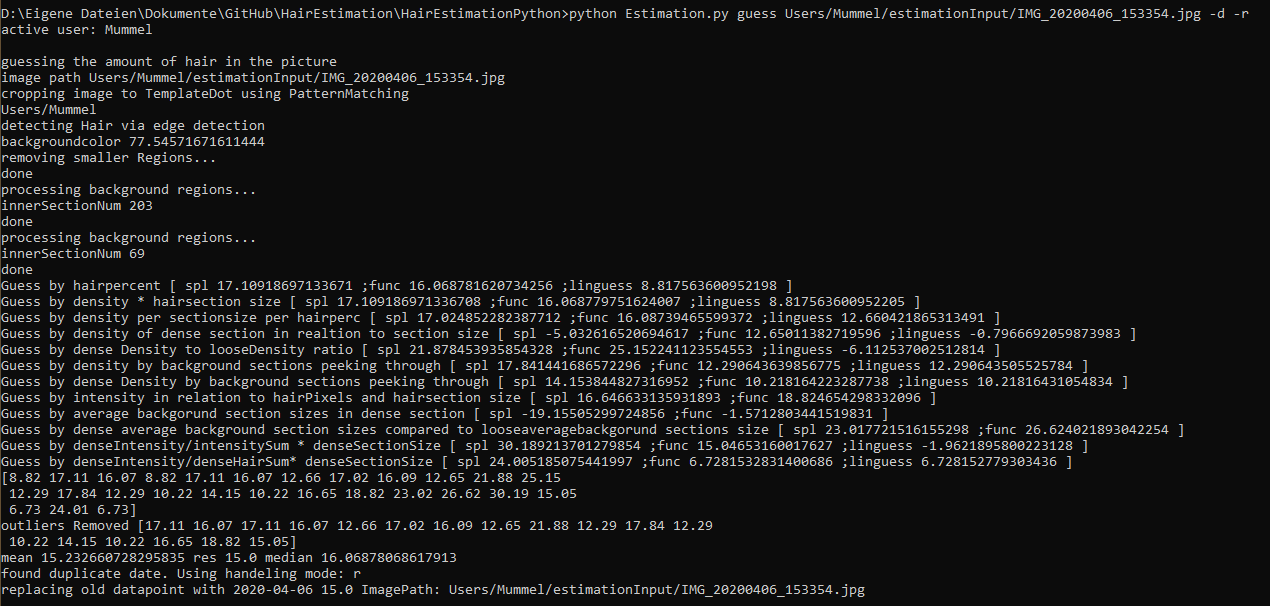
\includegraphics[width=1.1\textwidth]{fig64/commandlineGuessProcess.PNG}
  \caption[]{Kommandozeilenaufruf und Verlauf einer Schätzung}
  \label{comand:guess}
\end{figure} 

\subsection{Tests}
\subsection{Test: Knielange, dunkelrote Haare}

Knielange dunkelroten Haare wurden auf einem weißem Hintergrund aufgenommen. Die Ecken wurden mit dunkeln Punkten markiert. Siehe Abbildung \ref{img:tstM}.



es wurde eine Untersuchung in einem Zeitraum von 7 Wochen von dem tägliche Haarausfall angestellt. 
\begin{figure}
	\centering
	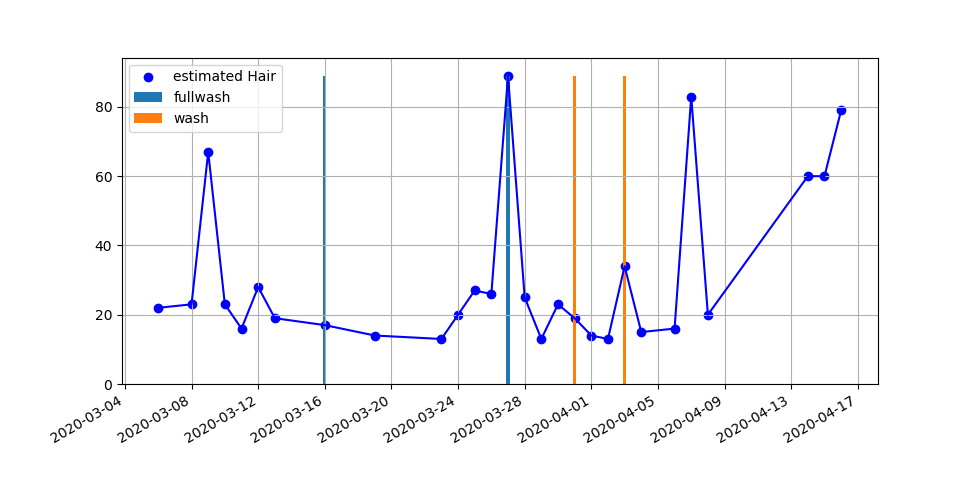
\includegraphics[width=1.0\textwidth]{fig64/plot.png}
	\caption[]{Schätzungen aus einem Zeitraum von 7 Wochen}
	\label{img:7weeks}
\end{figure} 

Um die Fehlerrate zu testen zu können wurde für einige der eingage Bilder die Anzahl der Haare per Hand gezählt.
Mit einer großen Menge an Kalibrations-Bildern konnten die folgenden Fehler in den Schätzungen vermerkt werden:
 
['15' '15' '18' '22' '22' '25' '30' '30' '37' '40' '60' '95'] calibration images
[27 22 23 22 67 17 23 16 28 19 17 14 13 20 27 26 89 25 13 23 19 14 13 34 estimated
21 16 56 27 20]
(estimated, actual)
[(27, 22), (22, 22), (23, 25), (22, 18), (67, 65), (17, 22), (23, 22), (16, 18), (28, 26), (19, 21), (17, 18), (14, 9), (13, 17), (20, 27), (27, 30), (26, 27), (89, 95), (25, 40), (13, 15), (23, 31), (19, 31), (14, 11), (13, 16), (34, 50), (21, 30), (16, 12), (56, 45), (27, 34), (20, 16)]
error per estimation [  5   0  -2   4   2  -5   1  -2   2  -2  -1   5  -4  -7  -3  -1  -6 -15
-2  -8 -12   3  -3 -16  -9   4  11  -7   4]


Mit nur 3 Kalibrationsbilern der Menge: 22, 60, 120 konnte diese Fehlerrate gefunden werden:

['15' '60' '95']
[30 26 25 23 81 14 22  9 33 17 12  9  8 19 24 28 94 26  7 23 16  6  6 39
18 10 62 31 19]
(estimated, actual)
[(30, 22), (26, 22), (25, 25), (23, 18), (81, 65), (14, 22), (22, 22), (9, 18), (33, 26), (17, 21), (12, 18), (9, 9), (8, 17), (19, 27), (24, 30), (28, 27), (94, 95), (26, 40), (7, 15), (23, 31), (16, 31), (6, 11), (6, 16), (39, 50), (18, 30), (10, 12), (62, 45), (31, 34), (19, 16)]
error per estimation [  8   4   0   5  16  -8   0  -9   7  -4  -6   0  -9  -8  -6   1  -1 -14
-8  -8 -15  -5 -10 -11 -12  -2  17  -3   3]
mean error 6.896551724137931
small calibration room

\subsection{Test: Hüftlange, feine, blonde Haare}

Blonde Haare wurden vor einem Schwarzen Hintergrund aufgenommen. 

\begin{figure*}
	\centering
	\begin{subfigure}[b]{0.475\textwidth}
		\centering
		\includegraphics[width=\textwidth]{testFig/B_IMG_20200322_093659_50.jpg}
		\caption[]{Geschätzt auf 23 Haare. Tatsächlich 25 Haare}
		\label{img:tstM1} 
	\end{subfigure}
	\hfill
	\begin{subfigure}[b]{0.475\textwidth} 
		\centering
		\includegraphics[width=\textwidth]{testFig/B_IMG_20200330_094438_20.jpg}
		\caption[]{Geschätzt auf 89 Haare. Tatsächlich 95.}
		\label{img:tstM2}
	\end{subfigure}
	\caption[  ]
	{\small Beispiel input von blonden langen Haaren} 
	\label{img:tstM}
\end{figure*}
Für den schwarzen Hintergrund wurde besonders matte schwarze Pappe verwendet. Wenn die Struktur der Pappe zu grob ist, oder durch einen Glanz der pappe sichbar wird, wir sie von der Canny Edge detection erkannt. 

Auf schwarzem Hintergrund ist Staub besonders gut sichtbar. Um die Wahrscheinlichkeit zu verringern, das Verschmutzungen auf der Pappe für die Markierungen in der Ecke gehalten werden, wurden die Markierungen von einem einfachen Punkt zu einem kreuz geändert.  

Mit ? Kalibrations-Bilder kann folgende Fehlerrate gefunden werden.
['10' '10' '10' '120' '124' '18' '20' '20' '25' '3' '30' '30' '30' '30'
'40' '5' '50' '51' '55' '70']
[ 4 10 30 44 50 24 24 71]
(estimated, actual)
[(4, 3), (10, 10), (30, 30), (44, 50), (50, 55), (24, 20), (24, 20), (71, 70)]
error per estimation [ 1  0  0 -6 -5  4  4  1]
mean error 2.625

Siehe Anhang B für Schätzungs modelle und die Verarbeitung von Blonden Haaren.


\subsection{Test: kurze Hellbraune Haare}

Für hellbraune haare hat es sich gezeigt, das ein schwarzen Hintergrund einen besseren Kontrast bietet.

\begin{figure*}
	\centering
	\begin{subfigure}[b]{0.475\textwidth}
		\centering
		
\includegraphics[width=\textwidth]{figJan/IMG_20200325_133957_10.jpg}
		\caption[]{Geschätzt auf ?? Haare. Tatsächlich 10 Haare}
		\label{img:tstJan1} 
	\end{subfigure}
	\hfill
	\begin{subfigure}[b]{0.475\textwidth} 
		\centering
		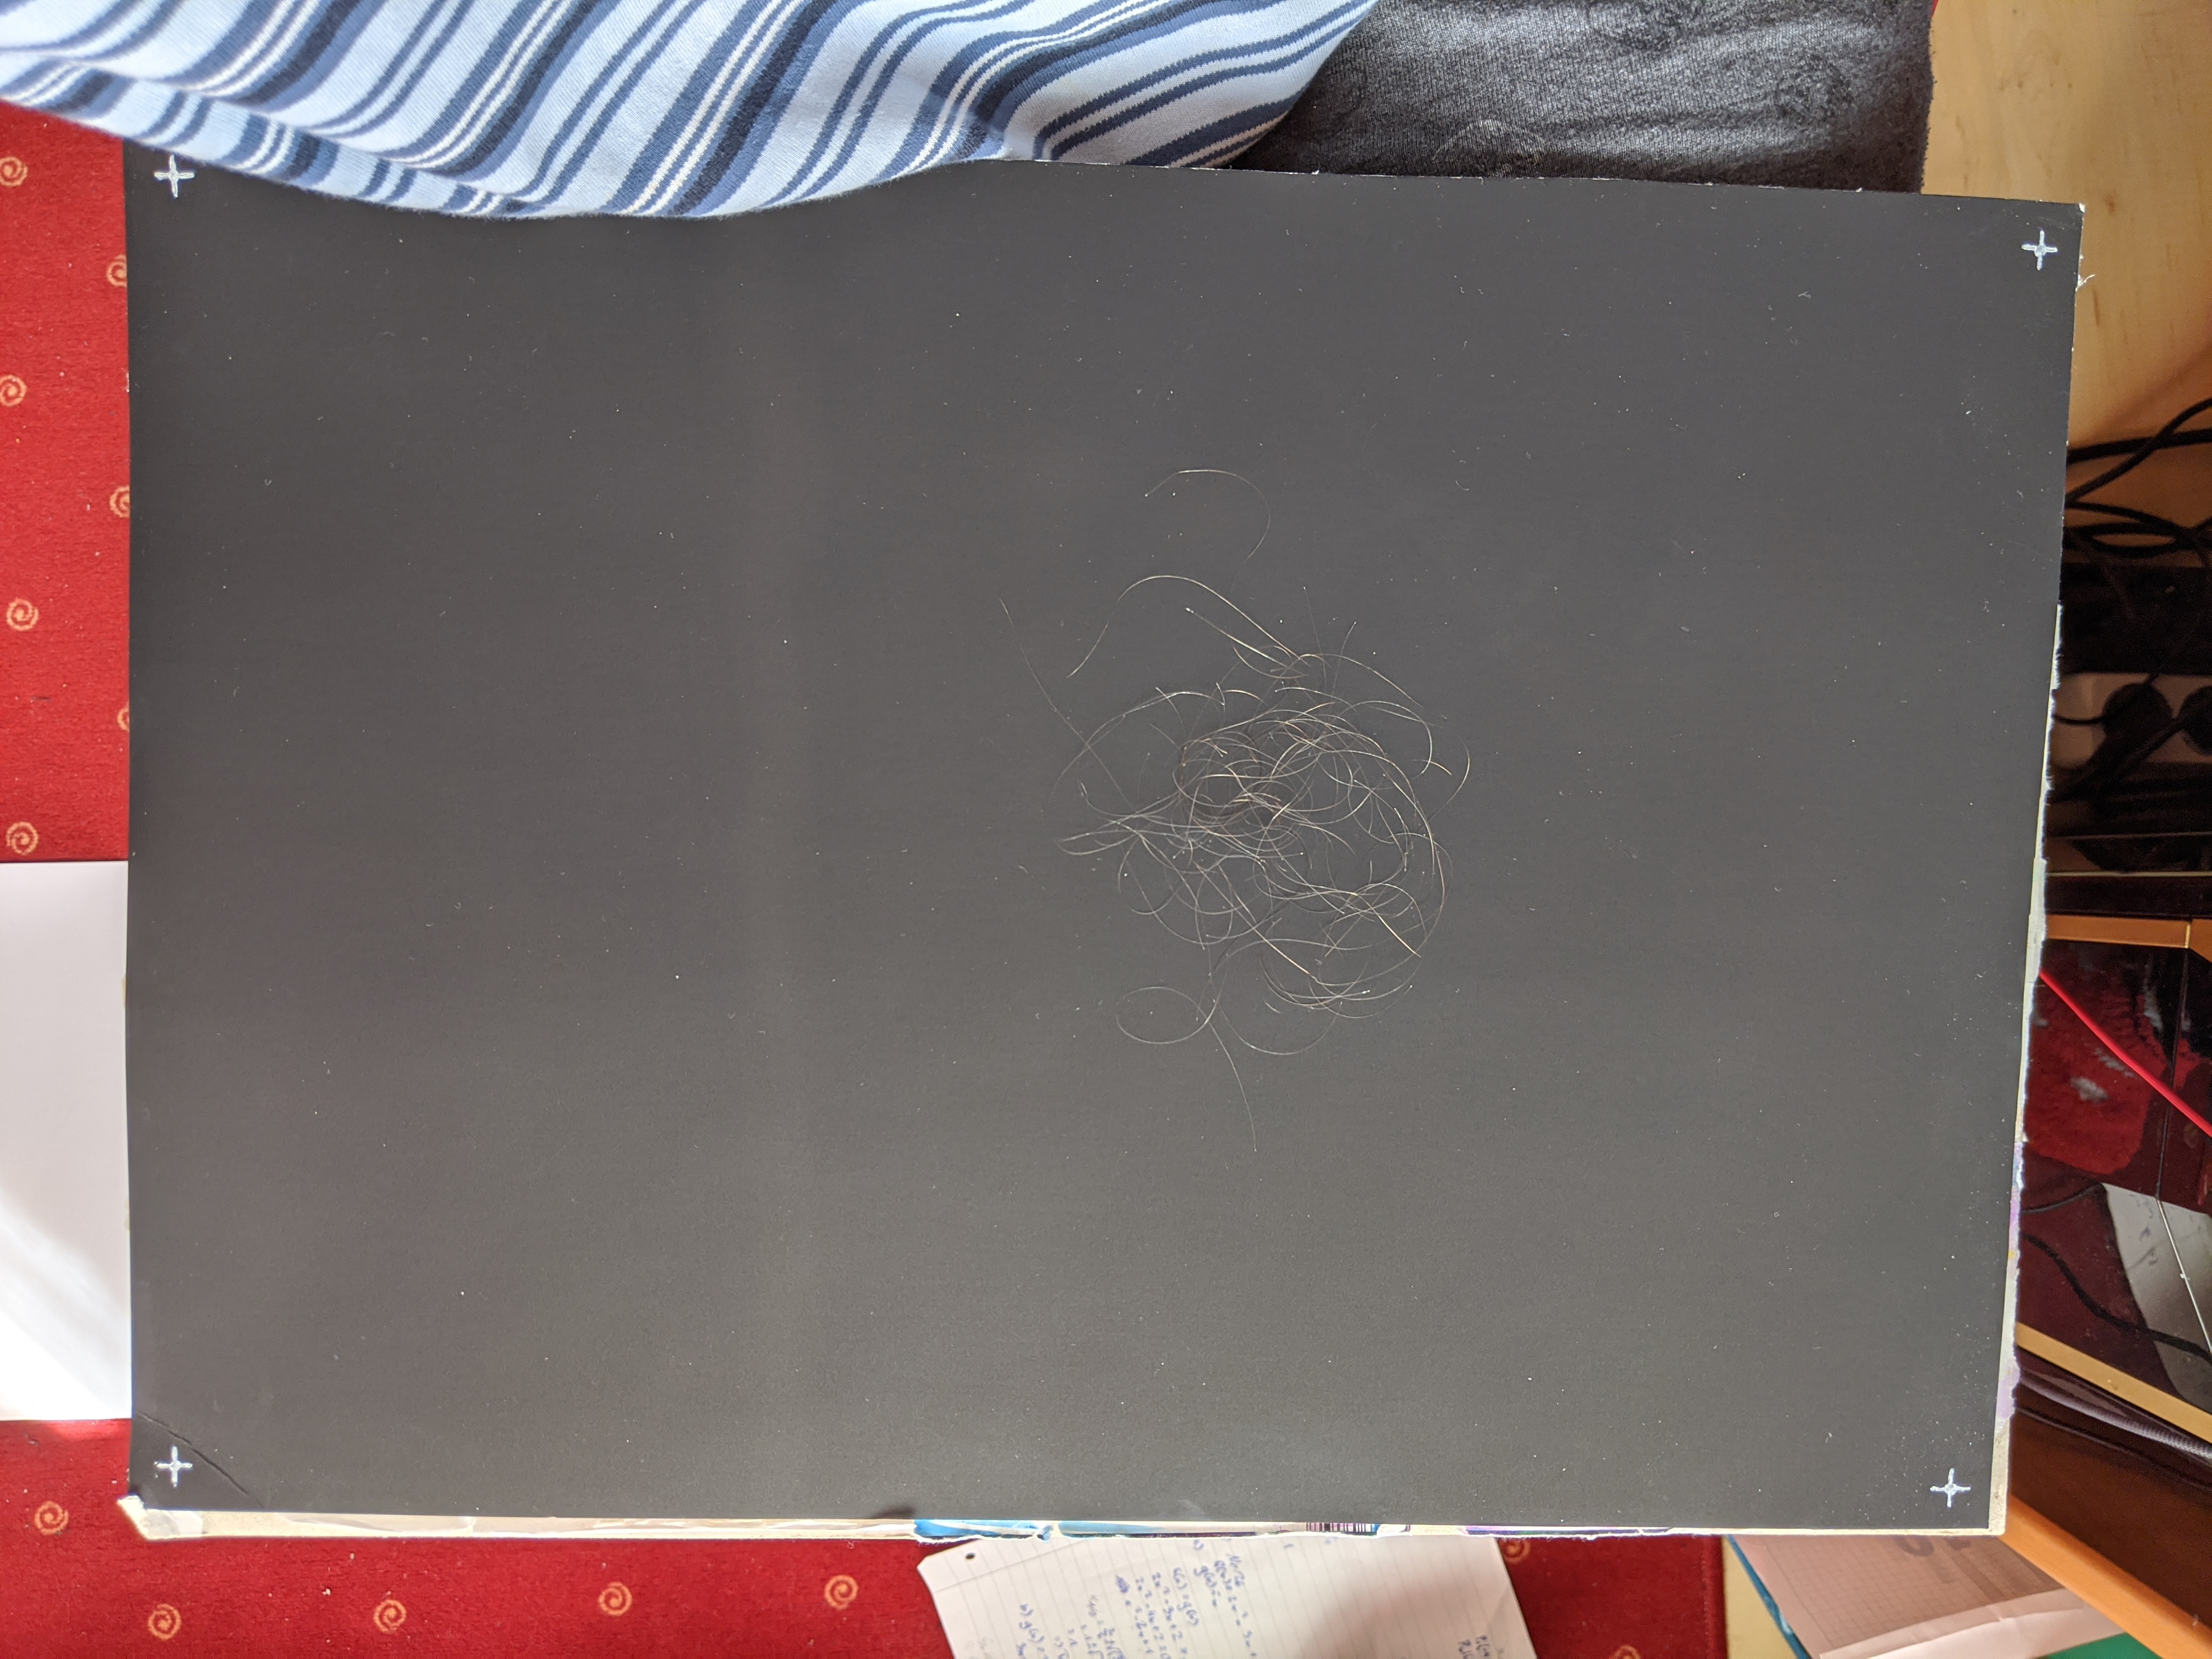
\includegraphics[width=\textwidth]{figJan/IMG_20200325_134247_40.jpg}
		\caption[]{Geschätzt auf ?? Haare. Tatsächlich 40.}
		\label{img:tstJan2}
	\end{subfigure}
	\caption[  ]
	{\small Beispiel input von blonden langen Haaren} 
	\label{img:tstJan}
\end{figure*}

Die Haare sind recht kurz und haben somit weniger Masse, im vergleich zu den vorherigen Testszenarien. Auch hier liegt die Fehlerrate bei :  

['10' '20' '40']
[ 8 10 14 20 16 31 36 40 37 10]
(estimated, actual)
[(8, 5), (10, 10), (14, 14), (20, 20), (16, 20), (31, 30), (36, 30), (40, 40), (37, 40), (10, 7)]
error per estimation [ 3  0  0  0 -4  1  6  0 -3  3]
mean error 2.0

\subsection{Test: Mama}
TODO

\section{Ergebnisse}
Durchschnittliche Fehler von 5 manchmal fehler von 10 Haaren. 
Da Haare manchmal mehr kürzere und manchmal mehr längere ausfallen kann man das nicht wirklich akkurat zählen. aber die generelle menge scheit gut geschätzt zu werden. 

ergebnisse more detailed als in dem paper. in dem paper wurde in inkrementen von 10, 50, 100, 200 etc gewertet. 

\section{Fazit}
Das Schätzen von Mengen an Haaren mithilfe von Bildverarbeitung und Statistischen Auswertungen zeigt sich als funktionsfähig und effizient. In der Zukunft können die unterschiedlichen Schäztungsmodelle miteinander verglichen werden, um die Kombination der akkuratesten Modelle zu finden. Und die Fehlerrate noch weiter zu reduzieren.
Des weiteren kann mit noch mehr Testsituationen mit unterschiedlichen Haar Typen aufgebaut werden. 

Die Bildverarbeitungs-prozess, besonders das Entfernen von kleinen Regionen und die Untersuchung der Hintergrundregionen dauert vergleichsweise lange (wie lange?? in ersten Test hinzufügen).  

%wird eine praktische Methode gegeben eine Langzeitüberwachung von Haarausfall anzustellen. So wird der Anwender sich bewusst, welcher tägliche Haarausfall normal ist und welche Menge besorgniserregend ist. Haarausfall ist sehr variabel und wird durch viele Faktoren beeinflusst. Eine Langzeitüberwachung beruhigt den Nutzer bei saisonalem Haarausfall und gibt Hinweise auf die allgemeine Gesundheit der Haare. Die Langzeitüberwachung macht den Haarausfall transparenter und berechenbarer. So wird der Nutzer früher aufmerksam auf anomalen Haarausfall und kann darauf besser reagieren. Haarverlust ist ein Indikator für viele Krankheiten und kann somit als Warnsystem dienen.

%\ref{cm}

%\begin{figure}
%	\centering
%	\includegraphics[width=0.7\textwidth]{PraiseMe_Prototyp4.jpg}
%	%\includegraphics[width=0.7\textwidth]{bild.jpg}
%	\caption[]{Cover des Spiels}
%	\label{img:cover}
%\end{figure}

%\section*{Gruppenmitglieder}

%\begin{itemize}
%	\item Umlauf, Niklas    -   3D-Artist
%\end{itemize}

%\nocite{reaper}
\newpage

\nocite{*}
\printbibliography



\appendix
\section{Anhang: 28 Datenpunkte pro Bild}
\label{appendix:datenpunkte}

\begin{itemize}
	\item intensitySum - Summe der Graustufenwerte des Intensität-Bildes
	\item intensityShare - Intensität pro HaarPixel
	\item hairpixels - Anzahl der Pixel, die Haare darstellen
	\item imagepixels - Gesammtanzahl der Pixel im Bild
	\item hairpixel percentage - Prozentsatz der Haarpixel im Bild
	\item number of sections - Anzahl an Hintergrund Regionen, die Watershed findet.
	\item number of background sections - Anzahl an Regionen, die den Hintergrund darstelle. (2 weniger als number of section. Watershed zählt Haare und übergänge zwischen Regionen mit)
	\item outerSectionSum - Summe an Pixeln, die sich in der Region befinden, die die Haare umschließt
	\item outerSectionPercentage - outerSectionSum/imagepixels
	\item innerSectionSum - Summa an Pixeln, die sich in Regionen befinden, die von Haaren umschlossen werden
	\item innserSectionAvgSize - Druchschnittliche Pixelanzahl, die sich in den umschlossenen Regionen befinden
	\item innerSectionAvgSize Percentage - innersectionAvgSize/imagepixels
	\item innerSectionSizeVariance - statistische Varianz der Pixelmengen, die sich in umschlossenen Regionen befinden
	\item innerSection standard deviation - Standardabweichung der Pixelmengen, die sich in umschlossenen Regionen befinden
	\item number of sections only concidering dense hair - Anzahl der Regionen, die Watershed findet nachdem der input Skelettiert wurde. Regionen werden von dichteren Haaren unterteilt.
	\item number of background sections inclosed by dense hair - Anzahl an Regionen, die den Hintergrund zwischen dichten Haaren darstellen
	\item dense hair outerSectionSum - Summe an Pixeln, die die Regionen umschließen, die von dichten Haaren umschlossen werden
	\item dense outerSectionPercentage - dense hair outerSectionSum / imagepixels
	\item dense innerSectionSum - Summe an Pixeln, die sich in den Regionen befinden, die von dichten Haaren umschlossen werden
	\item dense hair innserSectionAvgSize - Durschnittliche anzahl der Pixel, die sich in Regionen befinden, die von dichten Haaren umschlossen werden
	\item dense hair innerSectionAvgSize Percentage - dense hair innerSectionAvgSize / imagepixels
	\item dense innerSectionSizeVariance - statistische Varianz der Pixelmengen
	\item dense innerSection Size standard deviation - Standardabweichung der Pixelmengen
	\item denseHairSum - Summe an Pixeln, die als Dichte Haare angesehen werden
	\item looseHairSum - Summe an Pixeln, die als Haare angesehen werden, jedoch nicht als Dicht gelten
	\item IntensitySum in Loose Section - Summe der Graustufenwerte in nicht-dichten Regionen
	\item IntensitySum in Dense Section - Summe der Graustufenwerte in dichten Regionen
\end{itemize}

\section{Anhang x Wert berechungen für Schätzungs-Modelle}
\label{appendix:xwertemodel}
\begin{itemize}
	\item hairpercent 
	\begin{itemize}
		\item Prozentsatz der Haarpixel im Bild.
	\end{itemize}
	\item (hairpixels / hairSectionSize) * (1 - outerSectionPerc)
	\begin{itemize}
		\item HaarPixel Dichte in der Region, in der sich Haare Befinden. Gibt dasselbe Ergebnis wie hairpercent.
	\end{itemize}
	\item (hairpixels/hairSectionSize)*(1-outerSectionPerc)*hairPerc
	\item (((denseHairSum / denseInnerSectionSize) * (1 - denseSectionperc))) = denseDensity
	\begin{itemize}
		\item Dichte in den Dichten Regionen.
	\end{itemize}
	\item denseDensity / looseDensity
	\begin{itemize}
		\item Verhältnis dichte Regionen zu loosen Regionen.
	\end{itemize}
	\item backgroundSectionNum*(1-outerSectionPerc)
		\begin{itemize}
		\item Anzahl der HintergrundRegionen in Region, in der sich Haare Befinden.
	\end{itemize}
	\item denseSectionNum*(1-outerSectionPerc)
		\begin{itemize}
		\item Anzahl der HintergrundRegionen, die von dichten Haaren getrennt sind, in Haar-Region.
	\end{itemize}
	\item intensitySum*hairpixels*(1-outerSectionPerc)
	\begin{itemize}
		\item Intensitäts Summe pro HaarPixel in Haar-Region.
	\end{itemize}
	\item denseSectionAVGSize/(1-denseSectionperc)
		\begin{itemize}
		\item Durchschnittliche Größe der HintergrundRegionen, die durch dichte Haare getrennt sind.
	\end{itemize}
	\item (denseSectionAVGSize/looseSectionAVGSize)/(1-outerSectionPerc)
		\begin{itemize}
		\item Durchschnittliche Größe von Hintergrundregionen in dichten Regionen verglichen mit Durchschnittlicher Größe von Hintergrundregionen in loosen Regionen.
	\end{itemize}
	\item (denseIntensity/intensitySum)*(1-denseSectionperc)
		\begin{itemize}
		\item Intensität in Dichten Regionen verglichen mit gesammter Intensität.
	\end{itemize}
	\item (denseIntensity/denseHairSum)*(1-denseSectionperc)
		\begin{itemize}
		\item Intensität in Dichten Regionen verglichen mit Summe an Haarpixeln, die als dicht gelten.
	\end{itemize}
\end{itemize}

\section{Anhang Schätzungs Modelle}
\label{appendix:modelle}
\begin{figure}[H] % "[t!]" placement specifier just for this example
\begin{subfigure}{0.48\textwidth}
	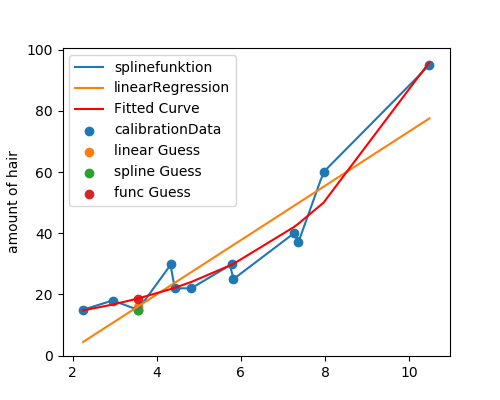
\includegraphics[width=1.1\linewidth]{fig64/g01_hairpercent.png}
	\caption{hairpercent} \label{fig:a}
\end{subfigure}\hspace*{\fill}
\begin{subfigure}{0.48\textwidth}
	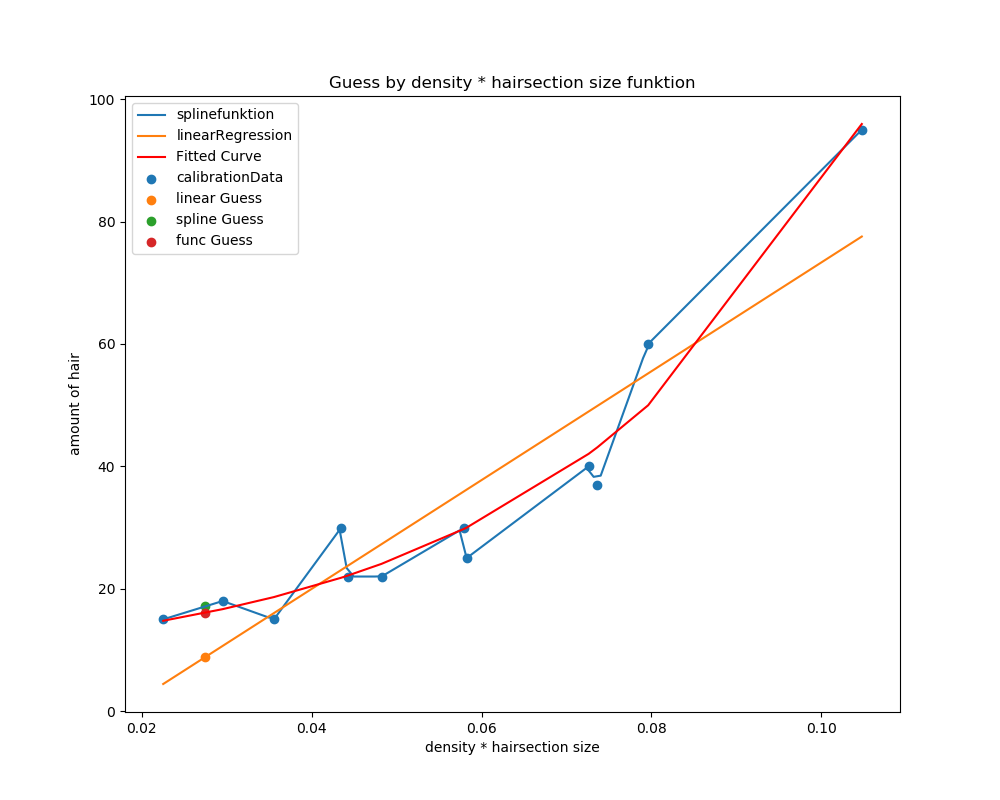
\includegraphics[width=1.1\linewidth]{fig64/g02_densitynorm.png}
	\caption{density*hairsection size} \label{fig:b}
\end{subfigure}

\medskip
\begin{subfigure}{0.48\textwidth}
	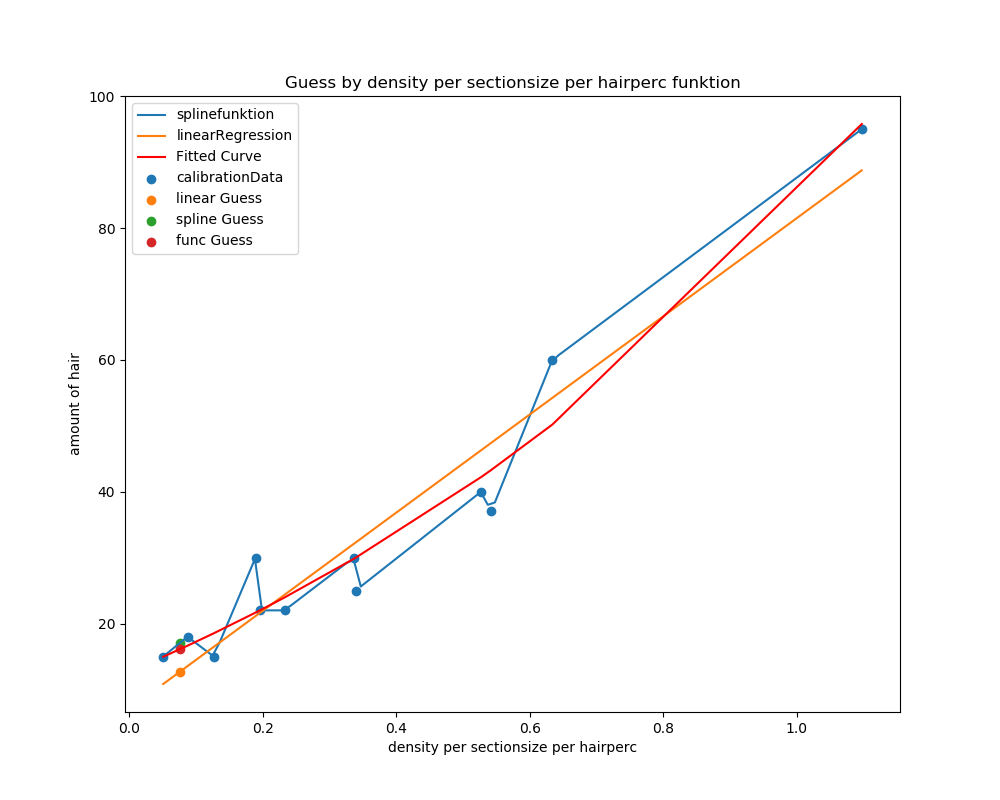
\includegraphics[width=1.1\linewidth]{fig64/g03_densitynorm2.png}
	\caption{density per sectionsize per hairperc} \label{fig:c}
\end{subfigure}\hspace*{\fill}
\begin{subfigure}{0.48\textwidth}
	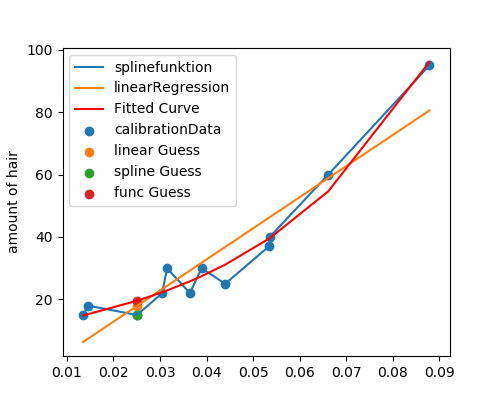
\includegraphics[width=1.1\linewidth]{fig64/g04_densityDenseSections.png}
	\caption{density of dense section in relation to section size} \label{fig:d}
\end{subfigure}

\medskip
\begin{subfigure}{0.48\textwidth}
	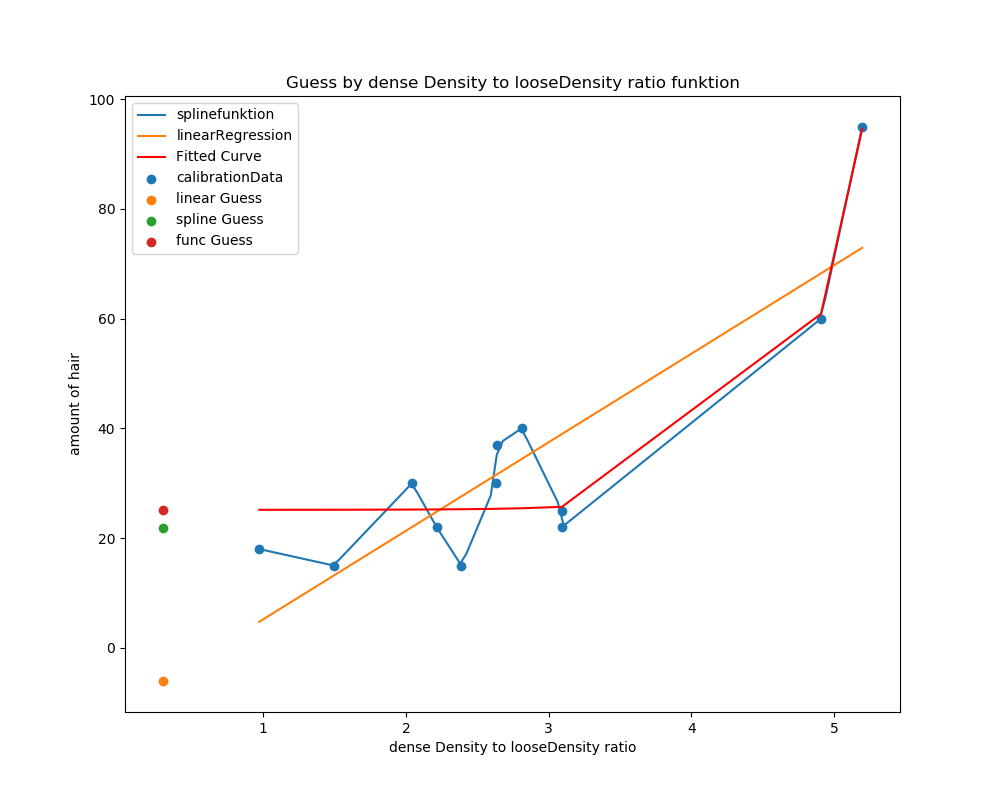
\includegraphics[width=1.1\linewidth]{fig64/g05_denseDensitytolooseDensity.png}
	\caption{dense Density to loose Density ratio} \label{fig:e}
\end{subfigure}\hspace*{\fill}
\begin{subfigure}{0.48\textwidth}
	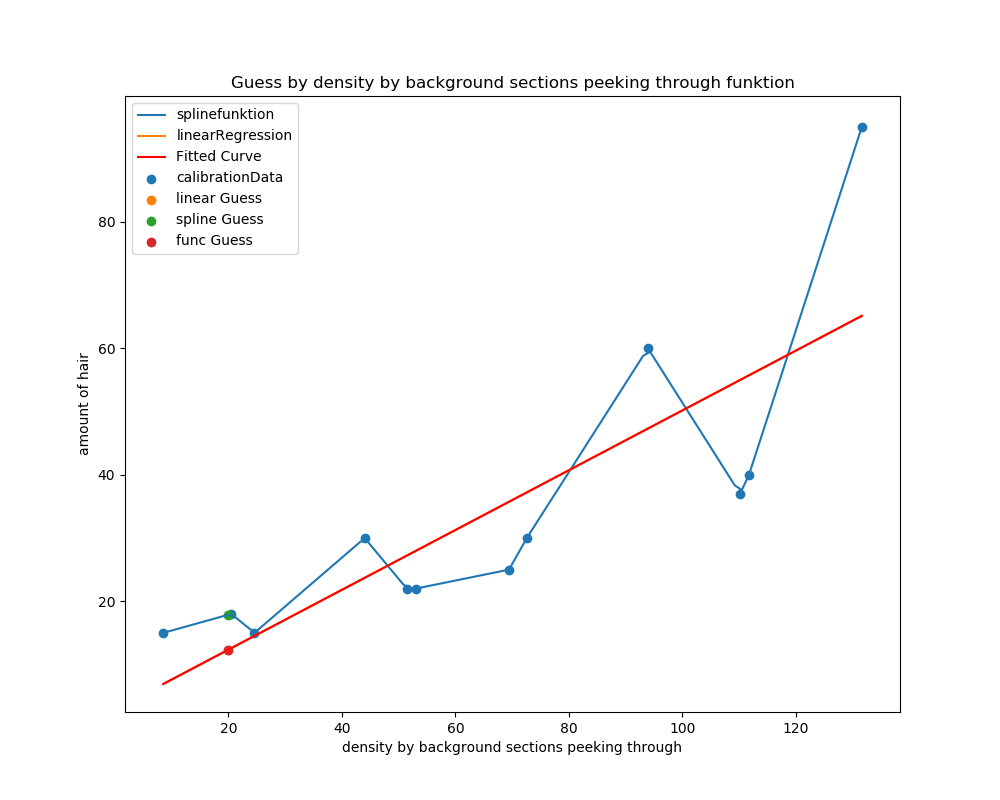
\includegraphics[width=1.1\linewidth]{fig64/g06_densitybybackgorundsections.png}
	\caption{density by background section peeking through} \label{fig:f}
\end{subfigure}


\caption{Schätzungsmodelle angewandt auf lange rotbraune Haare (1)} \label{fig:1}
\end{figure}

\begin{figure}[H] % "[t!]" placement specifier just for this example
	\begin{subfigure}{0.48\textwidth}
		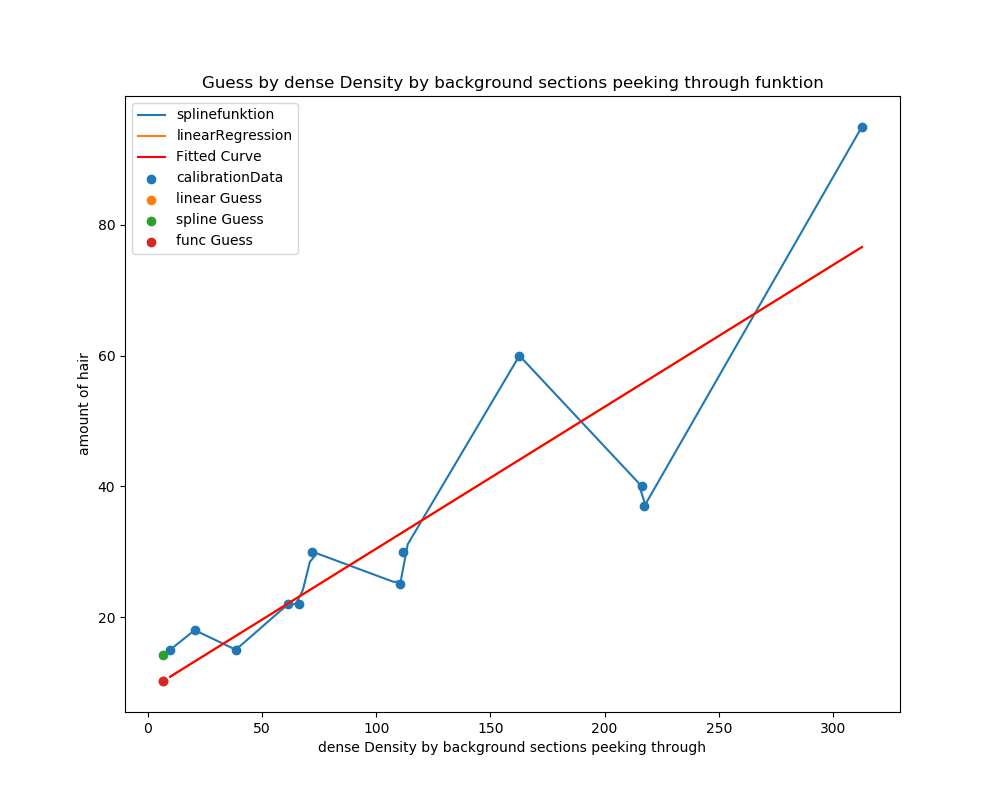
\includegraphics[width=1.15\linewidth]{fig64/g07_denseDensitybyBackgroundSections.png}
		\caption{dense Density by background section peeking through} \label{fig:a}
	\end{subfigure}\hspace*{\fill}
	\begin{subfigure}{0.48\textwidth}
		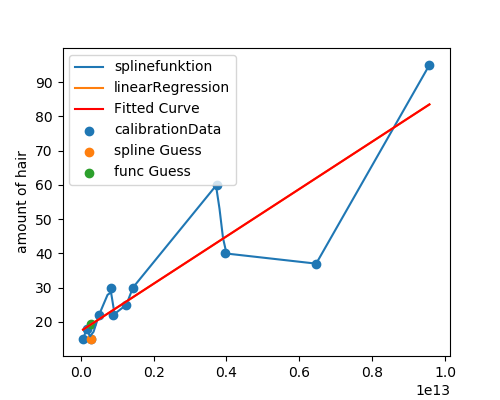
\includegraphics[width=1.15\linewidth]{fig64/g08_intensitynorm.png}
		\caption{intensity in relation to hairPixels and hairsectionsize} \label{fig:b}
	\end{subfigure}
	
	\medskip
	\begin{subfigure}{0.48\textwidth}
		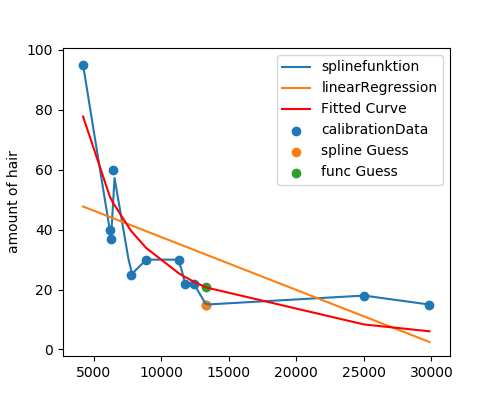
\includegraphics[width=1.15\linewidth]{fig64/g09_avgbackgroundsectionsizes.png}
		\caption{average background section sizes in dense section} \label{fig:c}
	\end{subfigure}\hspace*{\fill}
	\begin{subfigure}{0.48\textwidth}
		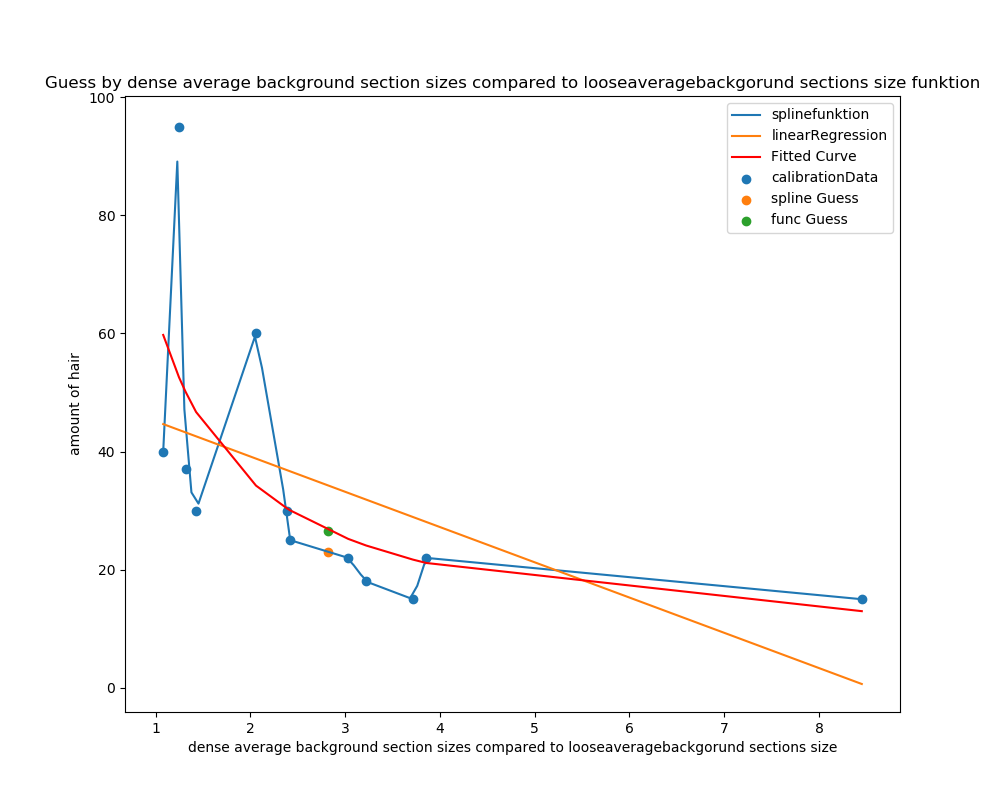
\includegraphics[width=1.15\linewidth]{fig64/g10_denseavgbackgroundsizeVSlooseavg.png}
		\caption{dense average background section size compared to looseaveragebackground section size} \label{fig:d}
	\end{subfigure}
	
	\medskip
	\begin{subfigure}{0.48\textwidth}
		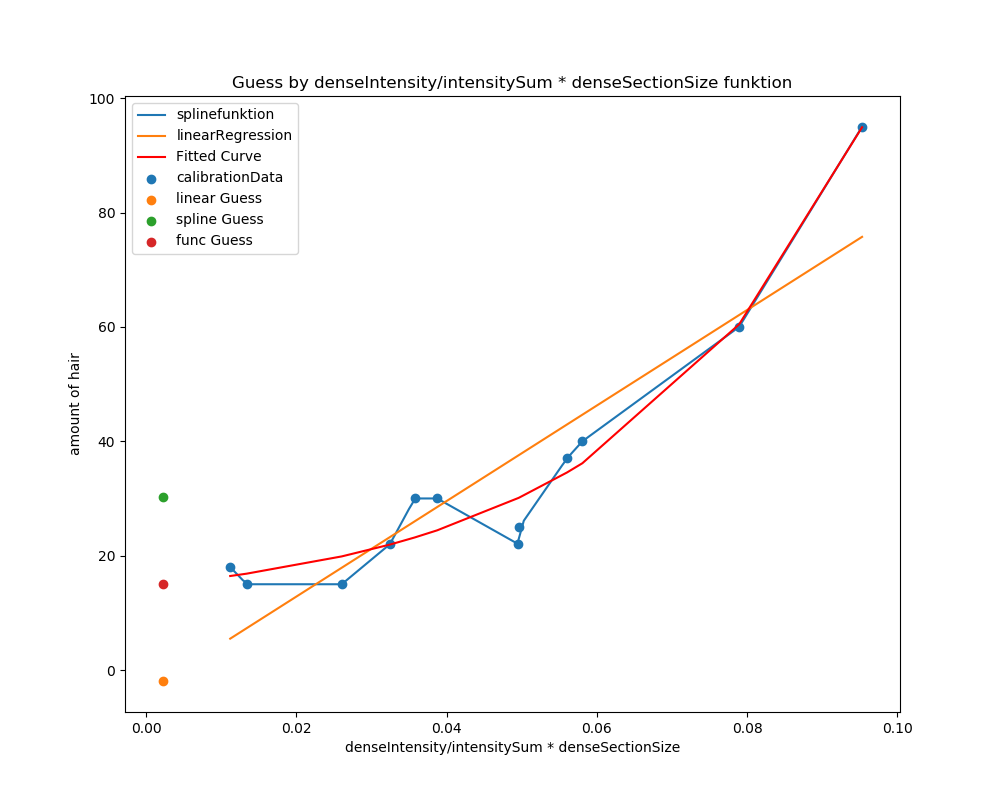
\includegraphics[width=1.15\linewidth]{fig64/g11_denseIntensitynorm.png}
		\caption{densityIntensity/intensitySum * denseSectionSize} \label{fig:e}
	\end{subfigure}\hspace*{\fill}
	\begin{subfigure}{0.48\textwidth}
		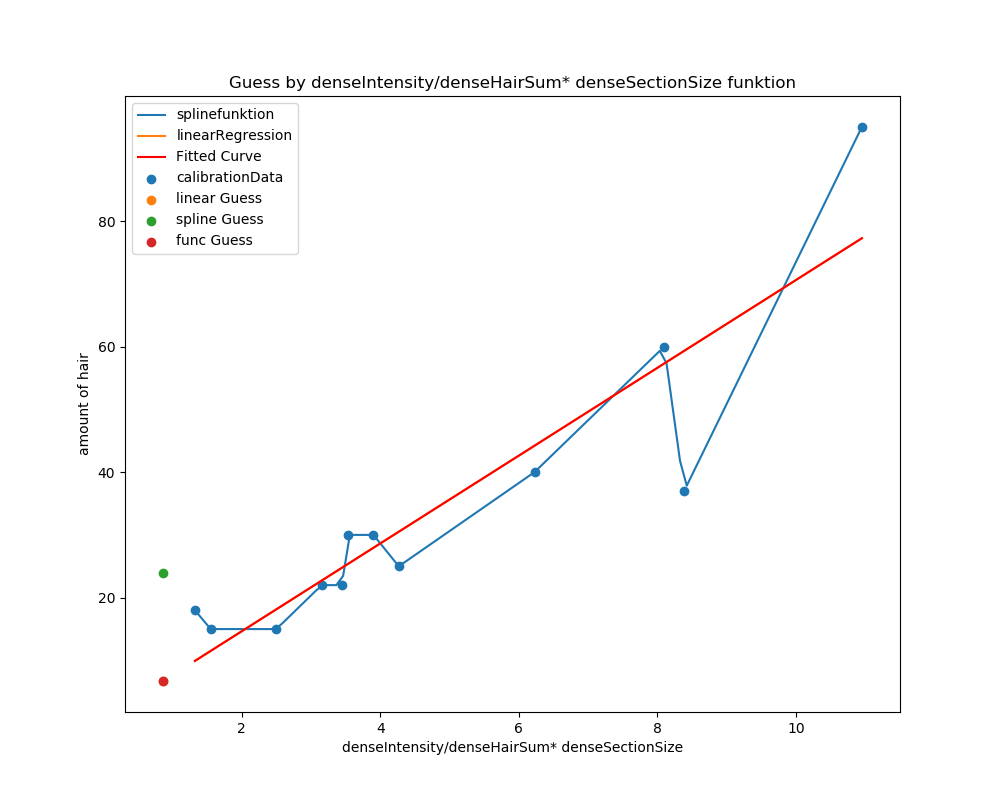
\includegraphics[width=1.15\linewidth]{fig64/g12_denseIntensitynorm2.png}
		\caption{denseIntensity/denseHairSum * denseSectionSize} \label{fig:f}
	\end{subfigure}
	
	
	\caption{Schätzngsmodelle angewandt auf lenge rotbraune Haare (2)} \label{fig:1}
\end{figure}

\section{Anhang: Blondes Haar}

\begin{figure}[H] % "[t!]" placement specifier just for this example
	\begin{subfigure}{0.48\textwidth}
		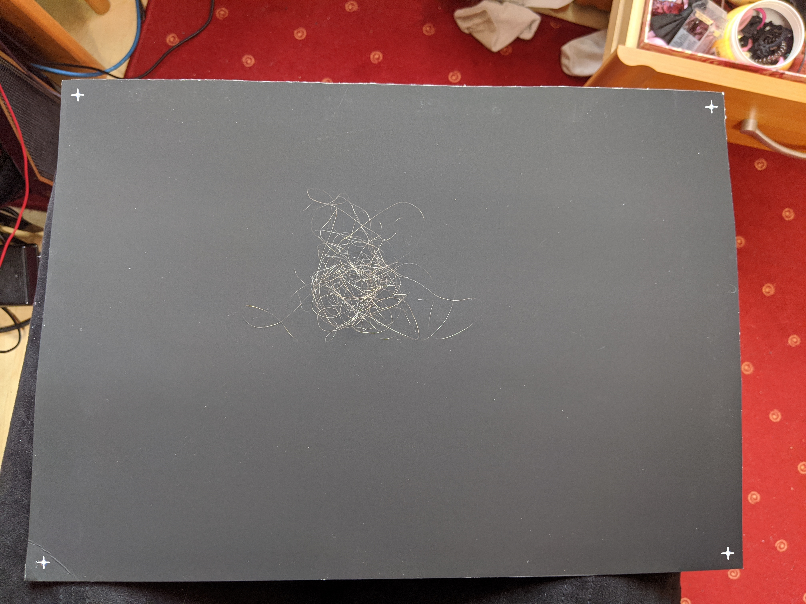
\includegraphics[width=\linewidth]{figBina/01foundDots.png}
		\caption{Input} \label{fig:a}
	\end{subfigure}\hspace*{\fill}
	\begin{subfigure}{0.48\textwidth}
		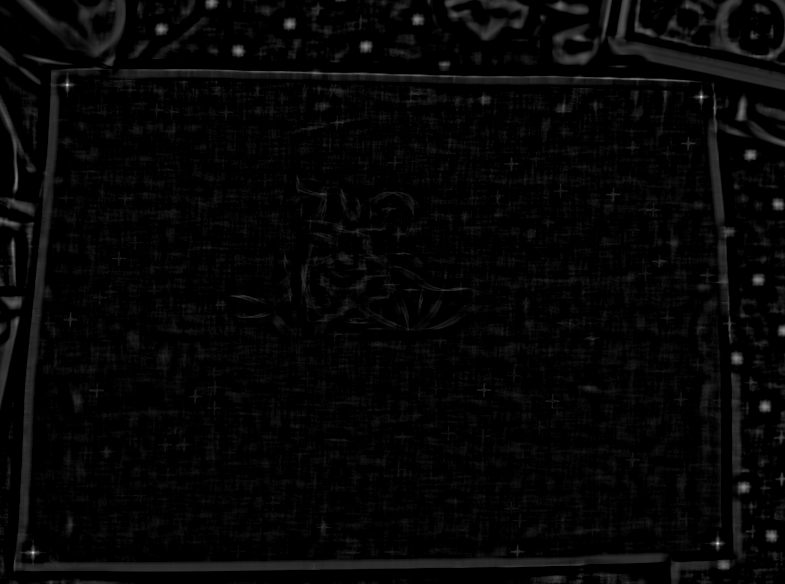
\includegraphics[width=\linewidth]{figBina/02revRes.png}
		\caption{Wahrscheinlichkeiten von matchTemplate} \label{fig:b}
	\end{subfigure}
	
	\medskip
	\begin{subfigure}{0.48\textwidth}
		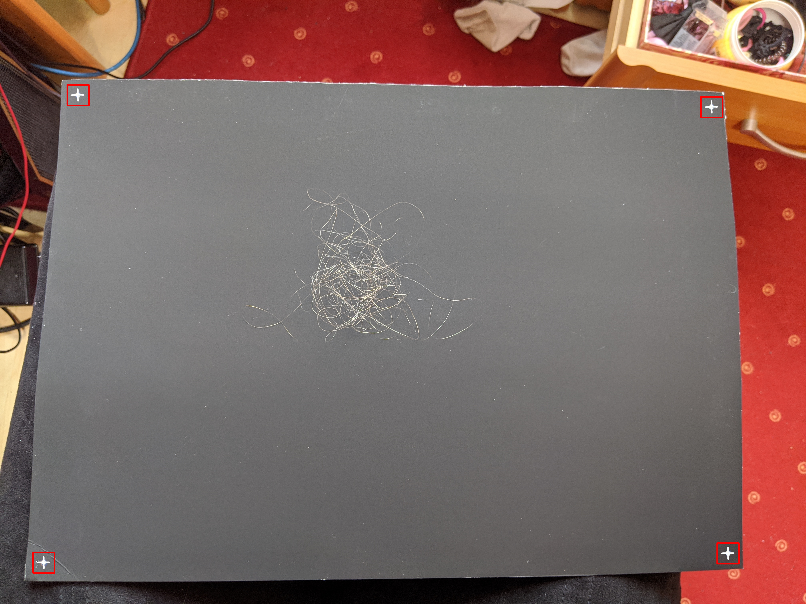
\includegraphics[width=\linewidth]{figBina/02foundDots.png}
		\caption{4 gefundene Markierungen} \label{fig:c}
	\end{subfigure}\hspace*{\fill}
	\begin{subfigure}{0.48\textwidth}
		
\includegraphics[width=\linewidth]{figBina/03crop image.png}
		\caption{Auf Markierungen zugeschnitten} \label{fig:d}
	\end{subfigure}
	
	\medskip
	\begin{subfigure}{0.48\textwidth}
		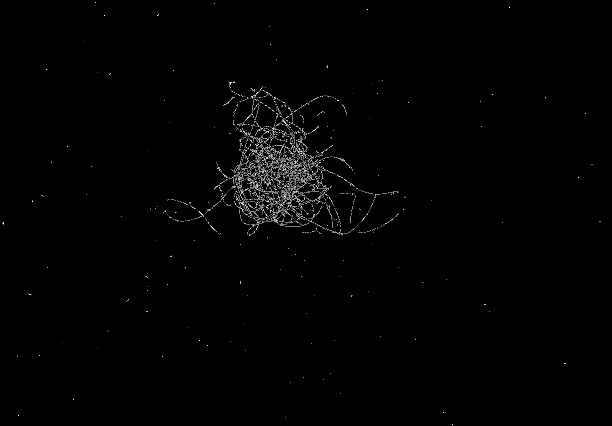
\includegraphics[width=\linewidth]{figBina/04edges.png}
		\caption{Kantendetektion} \label{fig:e}
	\end{subfigure}\hspace*{\fill}
	\begin{subfigure}{0.48\textwidth}
		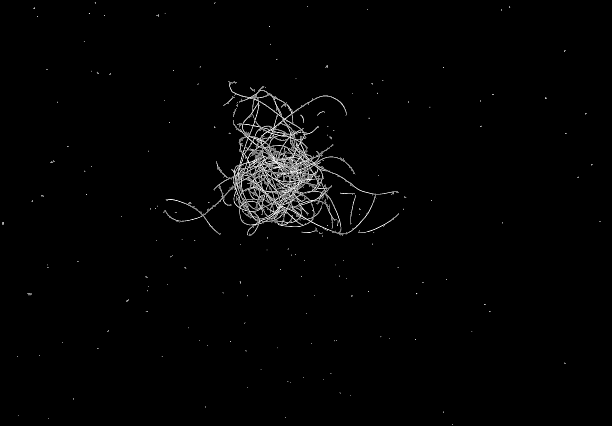
\includegraphics[width=\linewidth]{figBina/05intenstiy.png}
		\caption{Intensität} \label{fig:f}
	\end{subfigure}
	
	
	\caption{My complicated figure} \label{fig:1}
\end{figure}

\begin{figure}[H] % "[t!]" placement specifier just for this example
	\begin{subfigure}{0.48\textwidth}
		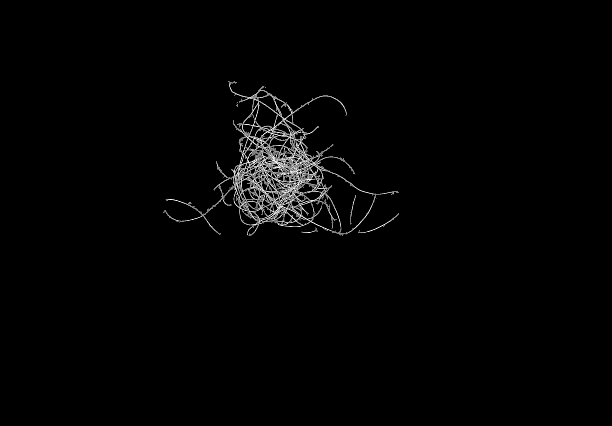
\includegraphics[width=\linewidth]{figBina/06small regions removed.png}
		\caption{Kleine Regionen entfernt} \label{fig:a}
	\end{subfigure}\hspace*{\fill}
	\begin{subfigure}{0.48\textwidth}
		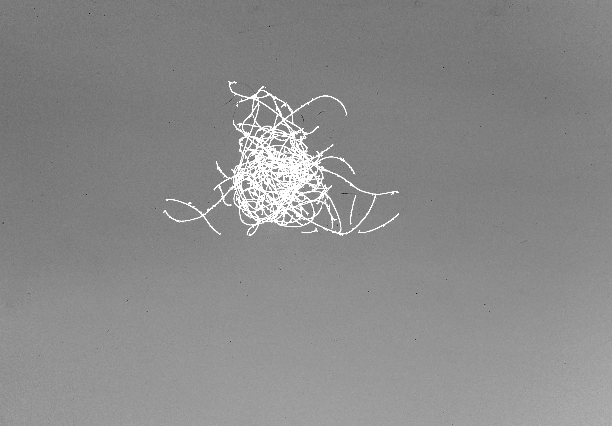
\includegraphics[width=\linewidth]{figBina/07missed hair.png}
		\caption{Intensität auf Input(Grayscale) ausgegeben. Zeigt wie viele Haare nicht erkannt wurden (hier: nicht viele)} \label{fig:b}
	\end{subfigure}
	
	\medskip
	\begin{subfigure}{0.48\textwidth}
		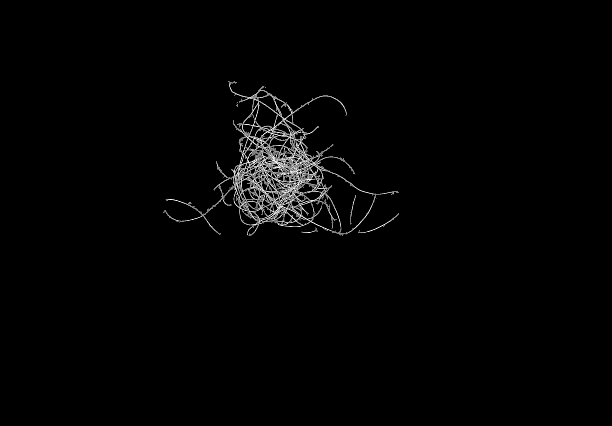
\includegraphics[width=\linewidth]{figBina/08input intensity.png}
		\caption{Intensität-Bild dient als Input für Hintergrund-Region-Untersuchung} \label{fig:c}
	\end{subfigure}\hspace*{\fill}
	\begin{subfigure}{0.48\textwidth}
		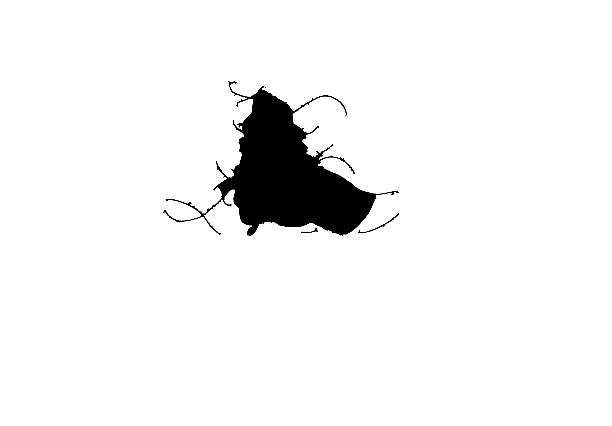
\includegraphics[width=\linewidth]{figBina/08outer section.png}
		\caption{Hintergrund Region, die die Haare umschließt, in weiß} \label{fig:d}
	\end{subfigure}
	
	\medskip
	\begin{subfigure}{0.48\textwidth}
		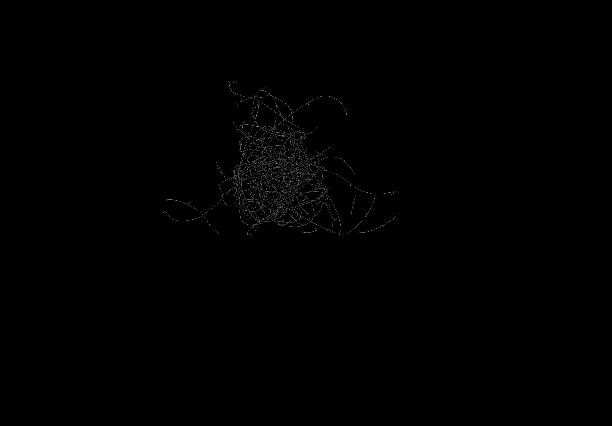
\includegraphics[width=\linewidth]{figBina/09input intensity.png}
		\caption{Intensität-Bild nach Skelettierung. Input für 2. Hintergrund Untersuchung} \label{fig:e}
	\end{subfigure}\hspace*{\fill}
	\begin{subfigure}{0.48\textwidth}
		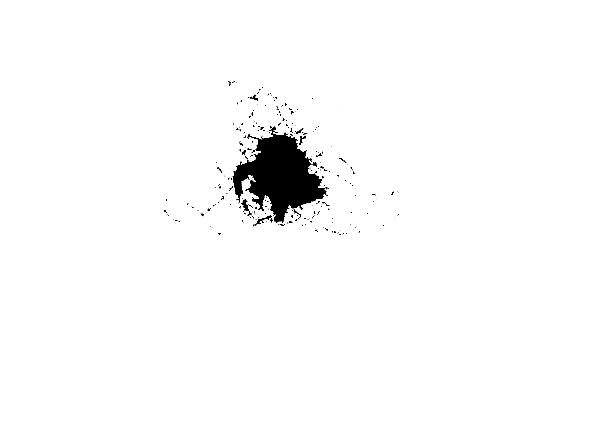
\includegraphics[width=\linewidth]{figBina/09outer section.png}
		\caption{Hintergrund Region, die dichte Haare umschließt} \label{fig:f}
	\end{subfigure}
	
	
	\caption{My complicated figure} \label{fig:1}
\end{figure}


\section{Anhang Schätzungs Modelle Blondes Haar}
\label{appendix:Blond}
\begin{figure}[H] % "[t!]" placement specifier just for this example
	\begin{subfigure}{0.48\textwidth}
		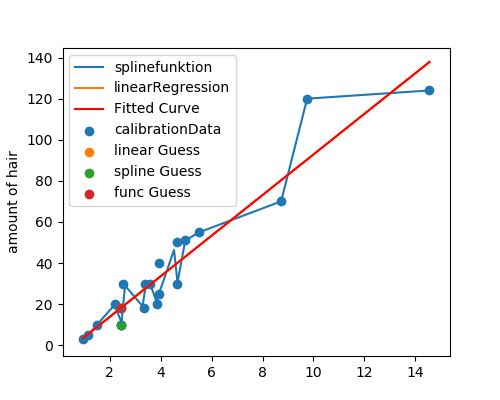
\includegraphics[width=1.1\linewidth]{figBina/g1.png}
		\caption{hairpercent} \label{fig:a}
	\end{subfigure}\hspace*{\fill}
	\begin{subfigure}{0.48\textwidth}
		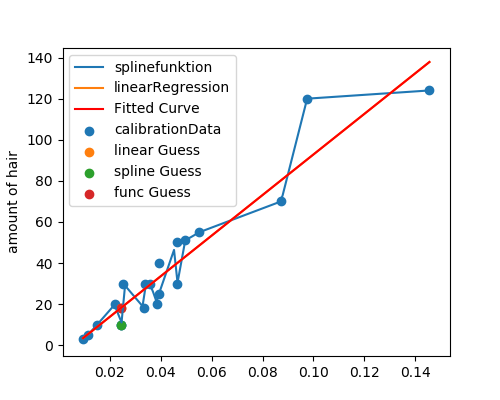
\includegraphics[width=1.1\linewidth]{figBina/g2.png}
		\caption{density*hairsection size} \label{fig:b}
	\end{subfigure}
	
	\medskip
	\begin{subfigure}{0.48\textwidth}
		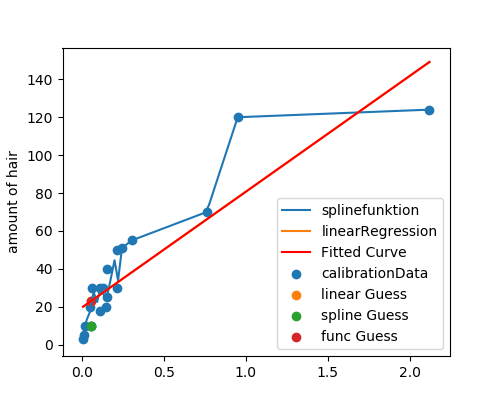
\includegraphics[width=1.1\linewidth]{figBina/g3.png}
		\caption{density per sectionsize per hairperc} \label{fig:c}
	\end{subfigure}\hspace*{\fill}
	\begin{subfigure}{0.48\textwidth}
		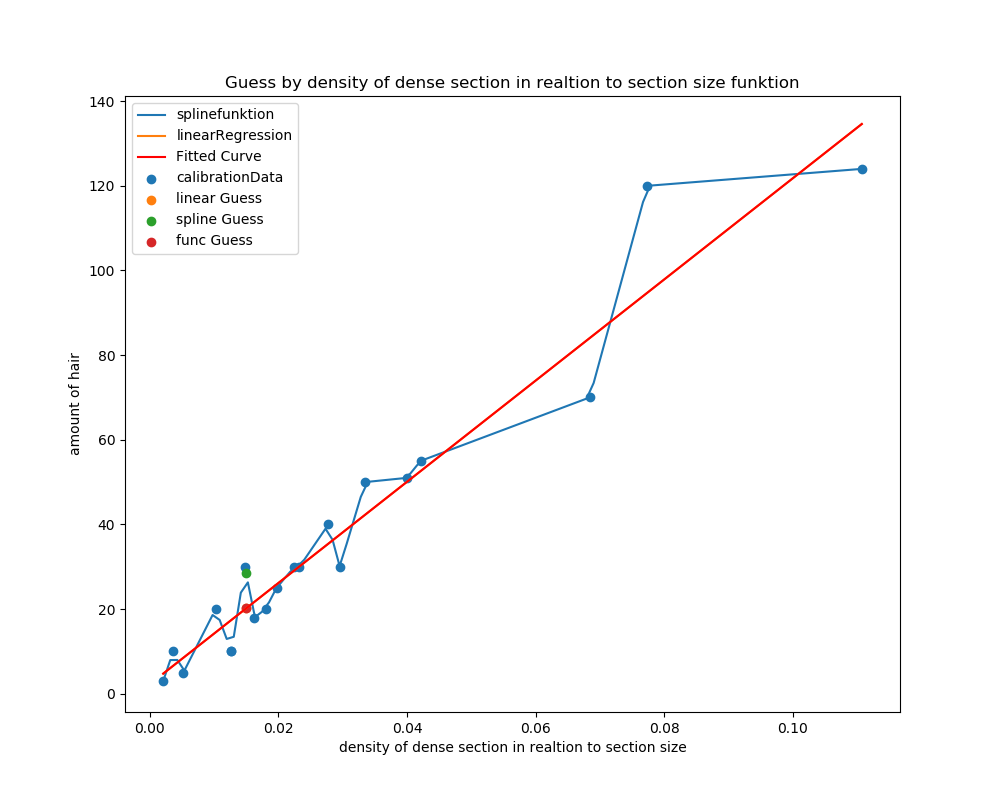
\includegraphics[width=1.1\linewidth]{figBina/g4.png}
		\caption{density of dense section in relation to section size} \label{fig:d}
	\end{subfigure}
	
	\medskip
	\begin{subfigure}{0.48\textwidth}
		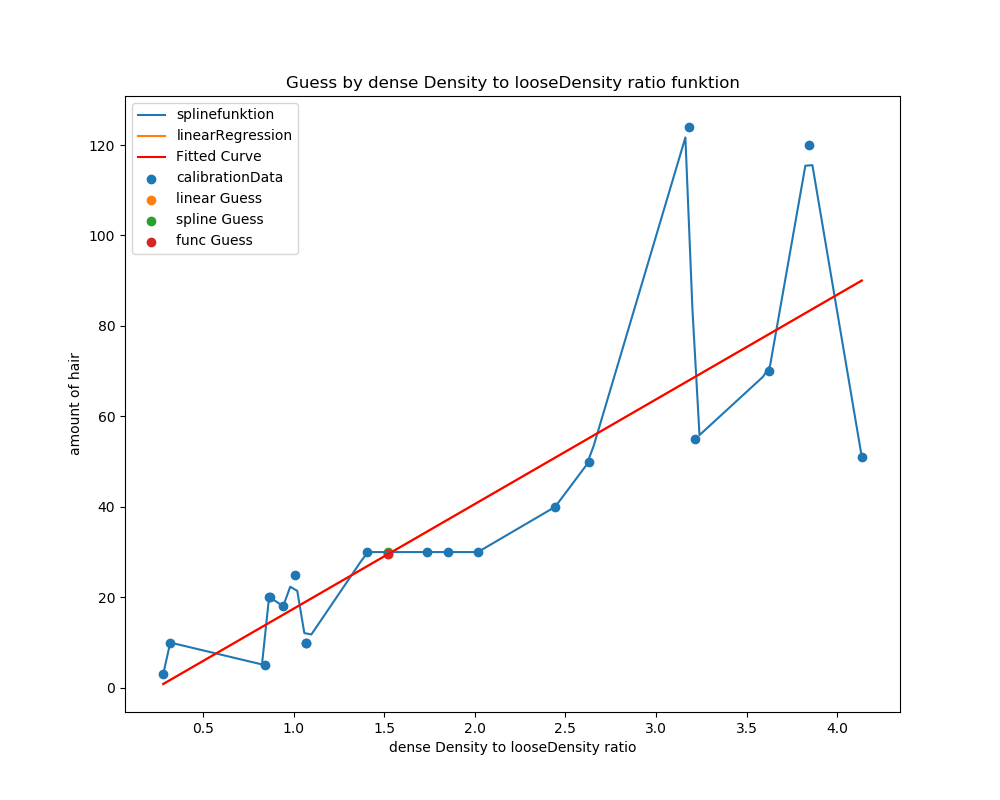
\includegraphics[width=1.1\linewidth]{figBina/g5.png}
		\caption{dense Density to loose Density ratio} \label{fig:e}
	\end{subfigure}\hspace*{\fill}
	\begin{subfigure}{0.48\textwidth}
		\includegraphics[width=1.1\linewidth]{figBina/g6.png}
		\caption{density by background section peeking through} \label{fig:f}
	\end{subfigure}
	
	
	\caption{Schätzungsmodelle angewandt auf feine blonde Haare (1)} \label{fig:1}
\end{figure}

\begin{figure}[H] % "[t!]" placement specifier just for this example
	\begin{subfigure}{0.48\textwidth}
		\includegraphics[width=1.1\linewidth]{figBina/g7.png}
		\caption{hairpercent} \label{fig:a}
	\end{subfigure}\hspace*{\fill}
	\begin{subfigure}{0.48\textwidth}
		\includegraphics[width=1.1\linewidth]{figBina/g8.png}
		\caption{density*hairsection size} \label{fig:b}
	\end{subfigure}
	
	\medskip
	\begin{subfigure}{0.48\textwidth}
		\includegraphics[width=1.1\linewidth]{figBina/g9.png}
		\caption{density per sectionsize per hairperc} \label{fig:c}
	\end{subfigure}\hspace*{\fill}
	\begin{subfigure}{0.48\textwidth}
		\includegraphics[width=1.1\linewidth]{figBina/g10.png}
		\caption{density of dense section in relation to section size} \label{fig:d}
	\end{subfigure}
	
	\medskip
	\begin{subfigure}{0.48\textwidth}
		\includegraphics[width=1.1\linewidth]{figBina/g11.png}
		\caption{dense Density to loose Density ratio} \label{fig:e}
	\end{subfigure}\hspace*{\fill}
	\begin{subfigure}{0.48\textwidth}
		\includegraphics[width=1.1\linewidth]{figBina/g12.png}
		\caption{density by background section peeking through} \label{fig:f}
	\end{subfigure}
	
	
	\caption{Schätzungsmodelle angewandt auf feine blonde Haare (2)} \label{fig:1}
\end{figure}



\end{document}